\graphicspath{{./fig_MM/}}


%
\section{単媒質の熱流動現象}

%
\subsection{支配方程式}

%
\subsubsection{熱伝導方程式と移流拡散方程式}
固体の熱伝導の支配方程式\cite{shouji:95:Dennetsu}は,

\begin{equation}
\rho^{\prime} C \frac{\partial \theta^{\prime}}{\partial t^{\prime}}
\, =\,
\frac{\partial}{\partial {x_{i}}^{\prime}} \left({ \lambda \frac{\partial \theta^{\prime}}{\partial {x_{i}}^{\prime}} }\right)\,+\, Q^{\prime}
\label{eq:heat conduction eq}
\end{equation}

\begin{center}
\begin{tabular}{lll}
$\rho^{\prime}$ &  $[kg/m^3]$ & density \\
$C$ & $[J/(kg\,K)]$ & specific heat\\
$\theta^{\prime}$ & $[K]$ & temperature \\
$\lambda$ & $[W/(m\,K)]$ & heat conductivity \\
$Q^{\prime}$ & $[W/m^3]$ & heat source\\
$t^{\prime}$ & $[s]$ & time\\
${u_{j}}^{\prime}$ & $[m/s]$ & velocity component \\
${x_{j}}^{\prime}$ & $[m]$ & coordinate axis\\
\end{tabular}
\end{center}

エネルギー方程式から非圧縮近似をして得られるパッシブスカラの移流拡散方程式は,

\begin{equation}
\rho^{\prime} C \,\left[{ \frac{\partial \theta^{\prime}}{ \partial t^{\prime}} \,+\, \frac{\partial}{\partial {x_{i}}^{\prime}} \,\left({{{u}'}_{i}\,{\mathit{\theta}}'}\right)}\right]
\, =\,
\frac{\partial}{\partial {x_{i}}^{\prime}} \,\left({ \lambda \frac{ \partial \theta^{\prime}}{\partial{x_{i}}^{\prime}} }\right) \,+\, {Q}^{\prime}
\label{eq:passive scalar eq}
\end{equation}

である.

%
\subsubsection{単媒質の場合の支配方程式}
有次元での計算は有効桁数の制約から桁落ちなどの問題が生じやすいため,$\theta \sim \mathrm{O}(1)$となるようにできるだけ無次元化して解きたい.\textbf{式(\ref{eq:passive scalar eq})}は次の代表値により無次元化される.

\begin{equation}
\left.{\begin{array}{l}
\vspace{1mm}
{u_{i}}^{\prime} \, = \,u_{\mathit{0}}^{\prime}\, u_{i}\\
\theta^{\prime} \, =\, {\theta_{\mathit{0}}}^{\prime} \,+\, \Delta \theta^{\prime} \, \theta\\
\vspace{1mm}
t^{\prime}\, =\, \left( {L}^{\prime} / {u_{\mathit{0}}}^{\prime} \right)\,t\\
\vspace{1mm}
{x_{i}}^{\prime} \, = \, L^{\prime} {x_{i}}
\end{array} \quad }\right\}
\label{eq:representative parameters}
\end{equation}

\begin{equation}
\frac{\mathrm{\partial}\mathit{\theta}}{\mathrm{\partial}{t}} \,+\, \frac{\mathrm{\partial}}{\mathrm{\partial}{x}_{i}}\hspace{0.15em}\left({{u}_{i} \hspace{0.15em} \mathit{\theta}}\right)
\, =\,
\frac{1}{Pe}\frac{\mathrm{\partial}}{\mathrm{\partial}{x}_{i}}\frac{\mathrm{\partial}\mathit{\theta}}{\mathrm{\partial}{x}_{i}} \,+\, {\mathrm{\Theta}}_{V}
\label{eq:passive scalar1 ND}
\end{equation}

\begin{equation}
\frac{1}{Pe} \,=\, \frac{\lambda}{\rho^{\prime} C} \frac{1}{{u_{\mathit{0}}}^{\prime} L^{\prime}}
\label{eq:passive scalar1-1 ND}
\end{equation}

\begin{equation}
\Theta_{V} \,=\, \frac{Q^{\prime}}{\rho^{\prime} C} \frac{L^{\prime}}{{u_{\mathit{0}}}^{\prime} \Delta \theta^{\prime}}
\label{eq:passive scalar1-2 ND}
\end{equation}

\noindent 対流項がない拡散場のみ,つまり熱伝導方程式の場合には,一般に熱輸送の時間スケール,代表速度は熱流の伝播速度に相当すると考え,

\begin{equation}
{u_{\mathit{0}}}^{\prime} \,= \,\frac{\alpha}{L^{\prime}}
\label{eq:velocity scale in natural convection}
\end{equation}

\noindent とスケーリングされる.この代表速度に基づき,Fourier数$F$を用いて均質場の熱輸送現象に適した無次元化が行われる.

\begin{equation}
{t} \,=\, \frac{{u_{\mathit{0}}}^{\prime}} {L^{\prime}}{t}^{\prime}
\,=\,
\frac{\alpha} {{L^{\prime}}^{2}} t^{\prime} \, \equiv\, {F}
\label{eq:scaling1:solid}
\end{equation}

\begin{equation}
\frac{\mathrm{\partial}\mathit{\theta}}{\mathrm{\partial}{F}}\,=\,\frac{\mathrm{\partial}}{\mathrm{\partial}{x}_{i}}\left({\frac{\mathrm{\partial}\mathit{\theta}}{\mathrm{\partial}{x}_{i}}}\right) \,+\, {W}{\mathrm{,}}\qquad
{W} \,=\, \frac{{L^{\prime}}^{2}}{\lambda \Delta \theta^{\prime}} Q^{\prime}
\label{eq:scaling2:solid}
\end{equation}

\noindent このとき,無次元化の代表時間スケール$\,{t_{0}}^{\prime}\,$は,
\begin{equation}
{t_{0}}^{\prime} \,=\, \frac{{L^{\prime}}^{2}}{\alpha} \qquad [s]
\label{eq:scaling1:time}
\end{equation}

\noindent 固体熱伝導を解く場合には,\textbf{式(\ref{eq:velocity scale in natural convection})}の代表速度を用いて\textbf{式(\ref{eq:passive scalar1 ND})}$\sim$\textbf{(\ref{eq:passive scalar1-2 ND})}を無次元化し,\textbf{式(\ref{eq:scaling2:solid})}と等価な解を得る.ただし,対流項の流体速度はゼロである.


%
\subsection{熱境界条件の種類と離散式への埋め込み}
\label{sec:heat_boundary}
%
\subsubsection{熱境界条件の種類と実装の指針}
C3Dソルバーでは,セル面に対して以下の熱境界条件を導入する.また,\textbf{式(\ref{eq:heat conduction eq})}の熱源$Q^{\prime}$は,セル体積に作用する境界条件として実装する.

\begin{equation}
\left.
\begin{array}{ll}
\vspace{2mm}
Adiabatic & q_{A}^{\prime}\,=\,0\\
\vspace{2mm}
Thermal\, conductivity & q_{C}^{\prime}\,=\,\displaystyle -\lambda\frac{\partial\theta^{\prime}}{\partial x_{i}^{\prime}}\\
\vspace{2mm}
Thermal\, transmission & q_{T}^{\prime}\,=\,-H(\theta_{s}^{\prime}-\theta_{\infty}^{\prime})\\
\vspace{2mm}
Thermal\, radiation & q_{R}^{\prime}\,=\,\sigma \varepsilon \left( {\theta_{s}^{\prime}}^{4} - {\theta_{\infty}^{\prime}}^{4} \right)\\
\vspace{2mm}
Isothermal & q_{ISO}^{\prime}\\
\vspace{2mm}
Direct & q_{D}^{\prime}
\end{array} \right\} \quad = \quad q_{BC}^{\prime}\quad [W/m^2]
\label{eq:thermal bc}
\end{equation}

\noindent 断熱条件は計算領域中の任意の場所で現れる可能性が可能性が高く,そのたびに境界条件処理を行うのはコストがかかる.これを回避するため,温度勾配をゼロにするマスク関数を基礎式中に導入することにより実装する.また,輻射はメカニズムが異なるので,他の熱境界条件の実装とは別に扱う.

残りのセル面に対する境界条件について,時間進行,あるいは反復過程での境界条件の導入方法を考える.空間インデクスのループを回し,その後に境界条件を設定すると,1ステップ/ループの遅れが生じる.境界条件のずれは,収束性の低下,あるいは解が異なる方向へ時間発展する可能性がある.また,ゴーストセルを導入した境界条件の設定は,圧力の場合と同様に多価の問題に厳密に対応する実装は難しい.
できるだけ現象にコンシステントな境界条件の導入を考えると,境界条件の導入レベルには以下の3つが考えられる.

\begin{enumerate}
\item 反復ループ内で,境界条件の時間遅れが無いように取り扱う.最も精確な方法は支配方程式に整合するように陰的にとり扱う方法であるが,実装は煩雑になる.
\item 一反復の遅れを許容すると,一反復前の物理量を用いて境界流束の評価を陽的に行え,実装が簡単になる.この場合,収束すると,ほぼ正しい境界条件になることが期待できる.
\item 1タイムステップ前の値を使う.1ステップの間の変化量が小さければ問題はなく,定常流解析では有効である.ソース項などに用いると,安定な傾向である.
\end{enumerate}

\noindent ここでは,2)の方法を採用し,ゴーストセルを使わず,簡単な形式かつ演算量の少ない方法でスキーム中に埋め込む方法を用いる.

熱境界条件を明示的に与えない固体-流体セル面\footnote{固体壁面の種類として,断熱壁面,熱伝導壁面,熱伝達壁面,等温壁面,熱流束指定面を設定できる.}は熱伝導面として扱う.熱伝導形式の境界条件は,基礎方程式中の拡散項で表現されているので,特別な境界条件を必要としない.\\

境界条件実装の方針をまとめると,以下のようになる.
\begin{itemize}
\item 境界熱流束$q_{BC}^{\prime}$の具体的な評価は,一反復前の値を用いて計算する.
\item 断熱は他の条件と排他的に扱い,基礎式に組み込む.
\item 熱伝導,熱伝達,等温,熱流束は各形式間で排他的に扱う.
\item 輻射は独立に考える.
\end{itemize}

これらのルールから,
\begin{equation}
{{q}'}_{BC}\,=\,
{\left[{\left({{{{q}'}_{ISO}}\,\vert\,
{{{q_T}'}\,\vert\,{{{q_C}'}}\,\vert\,{{q_D}'}}}\right)\,+\,{{q_R}'}}\right]}\,\vert\,{{{q_A}'}}
\label{eq:bc scheme}
\end{equation}

%
\subsubsection{スキームへの境界条件の埋め込み}
\label{sec:embbeded scheme}
\textbf{式(\ref{eq:bc scheme})}の境界条件をスキーム中に埋め込む実装方法として,境界条件マスク$\gamma_{BC}$と断熱マスク$\gamma_A$を導入する.境界条件マスクは通常の計算による熱流束と境界条件による熱流束を区別するために用いる.

\begin{equation}
\mathit{\gamma_{BC}}\,=\,\left\{
\begin{array}{lll}
0 & \mathrm{...} & BC\\
1 & \mathrm{...} & Non-BC
\end{array}
\right.
\label{eq:gamma BC definition}
\end{equation}

\begin{equation}
\mathit{\gamma_{A}}\,=\,\left\{
\begin{array}{lll}
0 & \mathrm{...} & Adiabatic\\
1 & \mathrm{...} & Non-adiabatic
\end{array}
\right.
\label{eq:gamma A definition}
\end{equation}

\noindent マスク関数を導入すると,拡散熱流束は次のように表記できる.

\begin{equation}
{q}_{i}^{\prime}\,=\,{\left[ \gamma_{A}\gamma_{BC} q^{\prime} \,+\, \gamma_{A}(1-\gamma_{BC}) q_{BC}^{\prime} \right]}_{i}
\label{eq:flux with gamma}
\end{equation}

\noindent マスクパターンと熱流束の対応は\textbf{表\ref{tbl:gamma table}}のようになる.

\begin{table}[htdp]
\caption{境界条件マスクによる熱境界条件パターン}
\begin{center}
\small
\begin{tabular}{lll}\toprule
$\gamma_{A}$ & $\gamma_{BC}$ & $q^{\prime}$\\ \midrule
0 & 0 & 0\\
0 & 1 & 0\\
1 & 0 & $q_{BC}^{\prime}$\\
1 & 1 & $q^{\prime}$\\ \bottomrule
\end{tabular}
\end{center}
\label{tbl:gamma table}
\end{table}%

\textbf{式(\ref{eq:passive scalar eq})}にEuler陽解法を適用し,空間項を有限体積的に評価すると,

\begin{equation}
\rho^{\prime}C \left[{\mathop{\int}\nolimits_{}{\frac{\mathrm{\partial}{\mathit{\theta}}'}{\mathrm{\partial}{t}'}}{d}{V}'\mathrm{{+}}\mathop{\int}\nolimits_{}{\frac{\mathrm{\partial}}{\mathrm{\partial} x_{i}^{\prime}}\left({{{u}_{i}}'{\mathit{\theta}}'}\right)}{d}{V}'}\right]
\,=\,
\mathrm{{-}}\mathop{\int}\nolimits_{}{\frac{\mathrm{\partial}{{q}'}_{i}}{\mathrm{\partial} x_{i}^{\prime}}}{d}{V}'\mathrm{{+}}\mathop{\int}\nolimits_{}{{Q}'}{d}{V}'
\label{eq:pscalar semi-discrete}
\end{equation}

\noindent 半離散的に示すと,

\begin{equation}
\rho^{\prime}C \frac{{\theta^{\prime}}^{n+1} - {\theta^{\prime}}^{n}} {\Delta t^{\prime}}
\,=\, -\, \frac{\rho^{\prime}C}{h^{\prime}} \sum\limits_{j=1}^{\dim\times2} {\left( u^{\prime}\,\theta^{\prime} \right)}_j \,n_j^{\prime}
\,- \frac{1}{h^{\prime}} \sum\limits_{j=1}^{\dim\times2} q_{j}^{\prime} \hspace{0.1em} n_{j}^{\prime} \,+\, Q^{\prime}
\label{eq:pscalar semi-discrete2}
\end{equation}

\noindent ここで,$ds^{\prime}$は法線成分をもつ面素,$n_{j}^{\prime}$はセルの外向き単位法線ベクトルである.右辺第二項を\textbf{式(\ref{eq:flux with gamma})}を用いて書き下すと,

\begin{equation}
- \frac{1}{h^{\prime}} \sum\limits_{j=1}^{\dim\times2} q_{j}^{\prime} \hspace{0.1em} n_{j}^{\prime}
\,=\,
- \frac{1}{h^{\prime}} \sum\limits_{j=1}^{\dim\times2} (-1)^{j} \left( \gamma_{A}\gamma_{BC} q^{\prime} \right)_{j} 
\,-\, 
\frac{1}{h^{\prime}} \sum\limits_{j=1}^{\dim\times2} (-1)^{j} \left\{ \gamma_{A} \left( 1-\gamma_{BC}\right) q_{BC}^{\prime} \right\}_{j}
\label{eq:pscalar semi-discrete3}
\end{equation}

\noindent 添字$j$は\textbf{図\ref{fig:cell index}}に示すように,着目するセルPを囲むセル(二次元では4つ,三次元では6つ)との界面を意味する.記号 \{w, e, s, n, b, t\} が $j=1\sim6$に対応する.一方,添字$J$は,\{W, E, S, N, B, T\} における物理量を表す.\textbf{式(\ref{eq:pscalar semi-discrete3})}の右辺第一項を書き下すと,

\begin{figure}[htdp]
\begin{center}
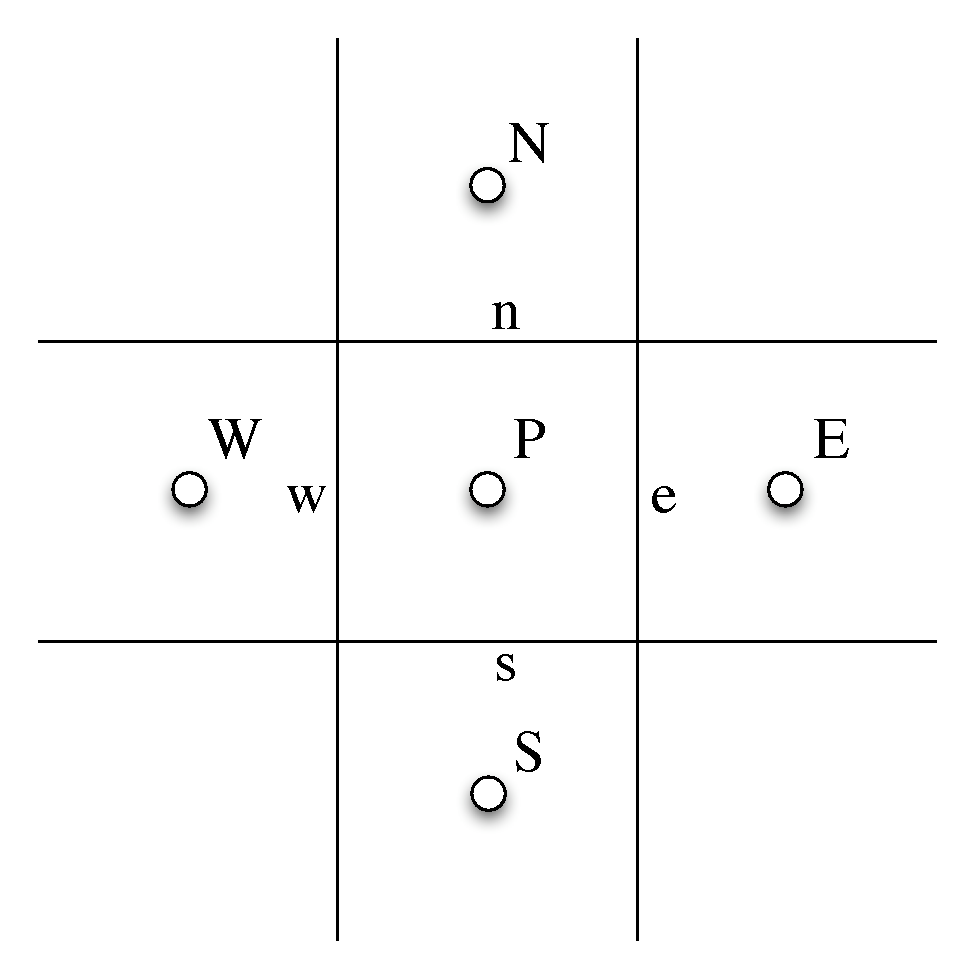
\includegraphics[width=5cm,clip]{index.eps}
\caption{更新セルと参照セルのインデクス}
\label{fig:cell index}
\end{center}
\end{figure}

\begin{equation}
- \frac{1}{h^{\prime}} \sum\limits_{j=1}^{\dim\times2} (-1)^{j} \left( \gamma_{A}\gamma_{BC} q^{\prime} \right)_{j}
\,=\,
\frac{1}{{h^{\prime}}^{2}} \sum\limits_{j=1}^{\dim\times2} \left( \gamma_{A}\gamma_{BC} \lambda \right)_{j} \left( \theta_{J}^{\prime} - \theta_{P}^{\prime} \right)
\,=\,
\frac{1}{{h^{\prime}}^{2}} \left[ \sum\limits_{j=1}^{\dim\times2} \left( \gamma_{A}\gamma_{BC} \lambda \right)_{j} \theta_{J}^{\prime} - 
\theta_{P}^{\prime} \sum\limits_{j=1}^{\dim\times2} \left( \gamma_{A}\gamma_{BC} \lambda \right)_{j} \right]
\label{eq:pscalar semi-discrete4}
\end{equation}

%
\begin{comment}
ここで多媒質の場合,界面における熱伝導率は次式を用いる.

\begin{equation}
\lambda_{j}^{\prime}
\,=\,
{2} \frac{\lambda_{J} \lambda_{P}} {\lambda_{J}^{\prime} + \lambda_{P}}
\label{eq:pscalar semi-discrete5}
\end{equation}
\end{comment}
%

\noindent したがって,\textbf{式(\ref{eq:pscalar semi-discrete2})}は

\begin{equation}
\begin{array}{l}
\displaystyle { \rho^{\prime}C \frac{ {\theta^{\prime}}^{\hspace{0.15em}n+1} - {\theta^{\prime}}^{\hspace{0.15em}n} } {\Delta t^{\prime}}
\,=\, 
-\, \frac{\rho^{\prime}C}{h^{\prime}} \sum\limits_{j=1}^{\dim\times2} {\left( u^{\prime}\,\theta^{\prime} \right)}_j \,n_j^{\prime}
\,+\,
\frac{1}{{h^{\prime}}^{2}} \left[ \sum\limits_{j=1}^{\dim\times2} \left( \gamma_{A}\gamma_{BC} \lambda \right)_{j} \theta_{J}^{\prime} 
\,-\, 
\theta_{P}^{\prime} \sum\limits_{j=1}^{\dim\times2} \left( \gamma_{A}\gamma_{BC} \lambda \right)_{j} \right] }\\
\displaystyle { \qquad \qquad \qquad \quad \,-\,
\frac{1}{h^{\prime}} \sum\limits_{j=1}^{\dim\times2} (-1)^{j} \left\{ \gamma_{A} \left( 1-\gamma_{BC} \right) q_{BC}^{\prime} \right\}_{j} \,+\, Q^{\prime} }
\end{array}
\label{eq:pscalar semi-discrete6}
\end{equation}


\noindent 無次元形式で表示すると,

\begin{equation}
\begin{array}{l}
\displaystyle { \frac{\theta^{\hspace{0.15em}n+1} - \theta^{\hspace{0.15em}n} } {\Delta t}
\, =\, -\, 
\frac{\rho C}{h} \sum\limits_{j=1}^{\dim\times2} {\left( u\,\theta \right)}_j \,n_j }\\
\displaystyle { \, + \,
\frac{1}{h^{2}Pe} \left[ \sum\limits_{j=1}^{\dim\times2} \left( {\gamma_{A}}_{j} {\gamma_{BC}}_{j} \theta_{J} \right)- \theta_{P} \sum\limits_{j=1}^{\dim\times2} {\gamma_{A}}_{j} {\gamma_{BC}}_{j} \right] 
\,-\,
\frac{1}{h} \sum\limits_{j=1}^{\dim\times2} (-1)^{j} \left\{ \left(1-\gamma_{A} \gamma_{BC} \right) q_{BC} \right\}_{j}
\,+\, \Theta_{V} }
\end{array}
\label{eq:pscalar semi-discrete7}
\end{equation}

\noindent ただし,

\begin{equation}
{q}_{BC} \,=\,\frac{q_{BC}^{\prime}} {u_{\mathit{0}}^{\prime} \Delta \theta^{\prime}} \frac{1}{\rho^{\prime}C}
\label{eq:qbc non-dimansionalize}
\end{equation}

である.このとき,無次元化パラメータに用いた$\rho^{\prime},\,C$は解くべき媒質の物性値であることに注意する.C3Dソルバークラスでは,XML入力ファイルにおいて,ReferenceセクションのRef\_IDタグでボクセルIDを指定する.このIDは,SteerセクションのModel\_Settingタグで媒質テーブルと対応づけられ,基礎式で解くべき媒質を示す.つまり,\textbf{式(\ref{eq:qbc non-dimansionalize})}の$\rho^{\prime},\,C$の媒質を示している.


%
\subsection{時間発展方程式}
基礎方程式\textbf{(\ref{eq:passive scalar1 ND})}の対流項を$F$でまとめて表し,時間進行スキームを切り替えるパラメータ$\alpha$を用いると,

\begin{equation}
{\frac{\partial \theta}{\partial t}}^{n+1}
\,=\,
\left({{1}\mathrm{{-}}\mathit{\alpha}}\right){F}^{\hspace{0.33em}{n}}\mathrm{{+}}\mathit{\alpha}{F}^{{n}\mathrm{{+}}{1}}\mathrm{{+}}{\mathrm{\Theta}}_{V}
\label{eq:pscalar evolv2}
\end{equation}

\begin{equation}
\alpha\,=\, \left\{
\begin{array}{cl}
0 & Euler\, Explicit\\
1/2 & Crank\, Nicolson\\
1 & Euler\, Implicit
\end{array} \right.
\label{eq:pscalar evolv3}
\end{equation}

\noindent ソース項の時制については任意性を残しておく.一般に時刻について線形化し,$\Theta_{V}^{\hspace{0.3em}n}$とする方が安定である.以下の議論では,拡散項の時間進行に着目して説明する.

%
\subsubsection{Euler陽解法}

\textbf{式(\ref{eq:pscalar semi-discrete7})}より,

\begin{equation}
\begin{array}{l}
\displaystyle { \frac{{\mathit{\theta}}_{P}^{\hspace{0.3em}{n}\mathrm{{+}}{1}}\mathrm{{-}}{\mathit{\theta}}_{P}^{\hspace{0.3em}{n}}}{\mathrm{\Delta}{t}}
\,=\, -
\frac{\rho C}{h} \sum\limits_{j=1}^{\dim\times2} {\left( u\,\theta \right)}_j \,n_j
\, + \,
\frac{1}{h^{2}Pe} \left[ \sum\limits_{j=1}^{\dim\times2} \left( {\gamma_{A}}_{j} {\gamma_{BC}}_{j} \theta_{J} \right)- \theta_{P} \sum\limits_{j=1}^{\dim\times2} {\gamma_{A}}_{j} {\gamma_{BC}}_{j} \right]^{n} }\\
\displaystyle { \,-\,
\frac{1}{h} \sum\limits_{j=1}^{\dim\times2} (-1)^{j} \left\{ \left(1-\gamma_{A} \gamma_{BC} \right) q_{BC} \right\}_{j}^{n}
\,+\, \Theta_{V}^{\hspace{0.3em}n} }
\end{array}
\label{eq:pscalar ee2}
\end{equation}

\noindent 陽解法の場合には,次の拡散数による数値安定性の点に注意する.
\begin{equation}
\Delta t \,\le\, \frac{1}{2dim}h^{2}Pe
\label{eq:pscalar ee3}
\end{equation}

%
\begin{comment}
\subsection{Euler陰解法}
\begin{equation}
{\frac{\mathrm{\partial}\mathit{\theta}}{\mathrm{\partial}{t}}}^{{n}\mathrm{{+}}{1}}
\,=\,
\mathrm{{-}}{\frac{\mathrm{\partial}{H}_{i}^{n+1}}{\mathrm{\partial}{x}_{i}}}^{n}\,\mathrm{{+}}\,{\mathrm{\Theta}}_{V}^{n}
\label{eq:pscalar ei1}
\end{equation}

\begin{equation}
\frac{{\mathit{\theta}}_{P}^{\hspace{0.33em}{n}\mathrm{{+}}{1}}\mathrm{{-}}{\mathit{\theta}}_{P}^{\hspace{0.33em}{n}}}{\mathrm{\Delta}{t}}\mathrm{{=}}\frac{1}{{h}^{2}Pe}{\left[{\mathop{\sum}\limits_{{j}\mathrm{{=}}{1}}\limits^{\dim\mathrm{\times}{2}}{\left({{\mathit{\gamma}}_{j}{\mathit{\theta}}_{J}}\right)}\mathrm{{-}}{\mathit{\theta}}_{P}\mathop{\sum}\limits_{{j}\mathrm{{=}}{1}}\limits^{\dim\mathrm{\times}{2}}{{\mathit{\gamma}}_{j}}}\right]}^{\hspace{0.33em}{n}\mathrm{{+}}{1}}\mathrm{{-}}\frac{1}{h}\mathop{\sum}\limits_{{j}\mathrm{{=}}{1}}\limits^{\dim\mathrm{\times}{2}}{\left[{{\mathrm{(}}\mathrm{{-}}{1}{\mathrm{)}}^{j}{\left\{{\left({{1}\mathrm{{-}}\mathit{\gamma}}\right){q}_{BC}}\right\}}_{j}^{\hspace{0.33em}{n}\mathrm{{+}}{1}}}\right]}\mathrm{{+}}{\mathrm{\Theta}}_{V}^{\hspace{0.33em}{n}}
\label{eq:pscalar ei2}
\end{equation}

反復式の形で対角項をまとめ,右肩の反復インデクスを$m$とすると,

\begin{equation}
\left[{{1}\mathrm{{+}}\frac{\mathrm{\Delta}{t}}{{h}^{2}Pe}\mathop{\sum}\limits_{{j}\mathrm{{=}}{1}}\limits^{\dim\mathrm{\times}{2}}{{\mathit{\gamma}}_{j}}}\right]{\mathit{\theta}}_{P}^{\hspace{0.33em}{m}\mathrm{{+}}{1}}\mathrm{{=}}{\mathit{\theta}}_{P}^{\hspace{0.33em}{n}}\mathrm{{+}}\frac{\mathrm{\Delta}{t}}{{h}^{2}Pe}\mathop{\sum}\limits_{{j}\mathrm{{=}}{1}}\limits^{\dim\mathrm{\times}{2}}{\left\{{{\mathit{\gamma}}_{j}{\mathit{\theta}}_{J}^{\hspace{0.33em}{m}\mathrm{{+}}{1}}}\right\}}\mathrm{{-}}\frac{\mathrm{\Delta}{t}}{h}\mathop{\sum}\limits_{{j}\mathrm{{=}}{1}}\limits^{\dim\mathrm{\times}{2}}{\left[{{\mathrm{(}}\mathrm{{-}}{1}{\mathrm{)}}^{j}{\left\{{\left({{1}\mathrm{{-}}\mathit{\gamma}}\right){q}_{BC}}\right\}}_{j}^{\hspace{0.33em}{m}}}\right]}\mathrm{{+}}\mathrm{\Delta}{t}\hspace{0.33em}{\mathrm{\Theta}}_{V}^{\hspace{0.33em}{n}}
\label{eq:pscalar ei3}
\end{equation}

右辺第二項の$q_{BC}$は一反復前の値を利用する.ソース項は,前の時刻の値か,あるいは前の反復値を用いる.

%
\subsection{Euler陰解法デルタ形式}
\begin{equation}
\begin{array}{l}
\displaystyle {\left[{{1}\mathrm{{+}}\frac{\mathrm{\Delta}{t}}{{h}^{2}Pe}\mathop{\sum}\limits_{{j}\mathrm{{=}}{1}}\limits^{\dim\mathrm{\times}{2}}{{\mathit{\gamma}}_{j}}}\right]\mathrm{\Delta}{\mathit{\theta}}_{P}^{{m}\mathrm{{+}}{1}}
\,=\,
\frac{\mathrm{\Delta}{t}}{{h}^{2}Pe}\mathop{\sum}\limits_{{j}\mathrm{{=}}{1}}\limits^{\dim\mathrm{\times}{2}}{\left({{\mathit{\gamma}}_{j}{\mathit{\theta}}_{J}^{{m}\mathrm{{+}}{1}}}\right)}\mathrm{{-}}\frac{\mathrm{\Delta}{t}}{h}\mathop{\sum}\limits_{{j}\mathrm{{=}}{1}}\limits^{\dim\mathrm{\times}{2}}{\left[{{\mathrm{(}}\mathrm{{-}}{1}{\mathrm{)}}^{j}{\left\{{\left({{1}\mathrm{{-}}\mathit{\gamma}}\right){q}_{BC}}\right\}}_{j}^{{m}}}\right]}}\\
\qquad \qquad \qquad \qquad \qquad \quad
\displaystyle {\mathrm{{-}}\left[{{1}\mathrm{{+}}\frac{\mathrm{\Delta}{t}}{{h}^{2}Pe}\mathop{\sum}\limits_{{j}\mathrm{{=}}{1}}\limits^{\dim\mathrm{\times}{2}}{{\mathit{\gamma}}_{j}}}\right]{\mathit{\theta}}_{P}^{{n}}\mathrm{{+}}\mathrm{\Delta}{t}{\mathrm{\Theta}}_{V}^{{n}}}
\end{array}
\label{eq:pscalar delta}
\end{equation}

%
\subsection{Crank-Nicolson}

\begin{equation}
{\frac{\mathrm{\partial}\mathit{\theta}}{\mathrm{\partial}{t}}}^{{n}\mathrm{{+}}{1}}
\,=\,
\mathrm{{-}}\frac{1}{2}\left({{\frac{\mathrm{\partial}{H}_{i}^{}}{\mathrm{\partial}{x}_{i}}}^{n}\mathrm{{+}}{\frac{\mathrm{\partial}{H}_{i}^{}}{\mathrm{\partial}{x}_{i}}}^{{n}\mathrm{{+}}{1}}}\right)\mathrm{{+}}{\mathrm{\Theta}}_{V}^{n}
\label{eq:pscalar cn1}
\end{equation}

\begin{equation}
\begin{array}{l}
\displaystyle {\left[{{1}\mathrm{{+}}\frac{\mathrm{\Delta}{t}}{2{h}^{2}Pe}\mathop{\sum}\limits_{{j}\,=\,{1}}\limits^{\dim\mathrm{\times}{2}}{{\mathit{\gamma}}_{j}}}\right]{\mathit{\theta}}_{P}^{{m}\mathrm{{+}}{1}}\,=\,{\mathit{\theta}}_{P}^{{n}}\mathrm{{+}}\frac{\mathrm{\Delta}{t}}{2{h}^{2}Pe}\mathop{\sum}\limits_{{j}\mathrm{{=}}{1}}\limits^{\dim\mathrm{\times}{2}}{\left({{\mathit{\gamma}}_{j}{\mathit{\theta}}_{J}^{{m}\mathrm{{+}}{1}}}\right)}\mathrm{{+}}\frac{\mathrm{\Delta}{t}}{2{h}^{2}Pe}{\left[{\mathop{\sum}\limits_{{j}\,=\,{1}}\limits^{\dim\mathrm{\times}{2}}{\left({{\mathit{\gamma}}_{j}{\mathit{\theta}}_{J}}\right)}\mathrm{{-}}{\mathit{\theta}}_{P}\mathop{\sum}\limits_{{j}\mathrm{{=}}{1}}\limits^{\dim\mathrm{\times}{2}}{{\mathit{\gamma}}_{j}}}\right]}^{{n}}}\\
\qquad \qquad \qquad \qquad \qquad
\displaystyle {\mathrm{{-}}\frac{\mathrm{\Delta}{t}}{2h}\left[{\mathop{\sum}\limits_{{j}\mathrm{{=}}{1}}\limits^{\dim\mathrm{\times}{2}}{\left\{{{\mathrm{(}}\mathrm{{-}}{1}{\mathrm{)}}^{j}{\left({\left({{1}\mathrm{{-}}\mathit{\gamma}}\right){q}_{BC}}\right)}_{j}^{n}}\right\}}}\right.\left.{\mathrm{{+}}\mathop{\sum}\limits_{{j}\mathrm{{=}}{1}}\limits^{\dim\mathrm{\times}{2}}{\left\{{{\mathrm{(}}\mathrm{{-}}{1}{\mathrm{)}}^{j}{\left({\left({{1}\mathrm{{-}}\mathit{\gamma}}\right){q}_{BC}}\right)}_{j}^{{m}}}\right\}}}\right]\mathrm{{+}}\mathrm{\Delta}{t}{\mathrm{\Theta}}_{V}^{{n}}}
\end{array}
\label{eq:pscalar cn2}
\end{equation}

%
\subsection{定常解}
\textbf{式(\ref{eq:pscalar evolv4})}を定常状態として計算する場合には,次式を解く.

\begin{equation}
{\mathit{\theta}}_{P}^{{m}\mathrm{{+}}{1}}
\,=\,
{\left[{\mathop{\sum}\limits_{{j}\mathrm{{=}}{1}}\limits^{\dim\mathrm{\times}{2}}{{\mathit{\gamma}}_{j}}}\right]}^{\mathrm{{-}}{1}}\left[{\mathop{\sum}\limits_{{j}\mathrm{{=}}{1}}\limits^{\dim\mathrm{\times}{2}}{\left({{\mathit{\gamma}}_{j}{\mathit{\theta}}_{J}^{{m}\mathrm{{+}}{1}}}\right)}\mathrm{{-}}{hPe}\mathop{\sum}\limits_{{j}\mathrm{{=}}{1}}\limits^{\dim\mathrm{\times}{2}}{\left\{{{\mathrm{(}}\mathrm{{-}}{1}{\mathrm{)}}^{j}{\left({\left({{1}\mathrm{{-}}\mathit{\gamma}}\right){q}_{BC}}\right)}_{j}^{{m}}}\right\}}\mathrm{{-}}{h}^{2}{Pe}{\mathrm{\Theta}}_{V}^{{n}}}\right]
\label{eq:pscalar steady}
\end{equation}

この場合$\gamma$の状況により対角項の係数がゼロになる場合が生じる.この問題点を回避するために,圧力の場合と同様に$\varepsilon$を導入する.

\begin{equation}
{\mathit{\theta}}_{P}^{{m}\mathrm{{+}}{1}}
\,=\,
{\left[{\mathrm{\varepsilon}\mathrm{{+}}\mathop{\sum}\limits_{{j}\mathrm{{=}}{1}}\limits^{\dim\mathrm{\times}{2}}{{\mathit{\gamma}}_{j}}}\right]}^{\mathrm{{-}}{1}}\left[{\mathop{\sum}\limits_{{j}\mathrm{{=}}{1}}\limits^{\dim\mathrm{\times}{2}}{\left({{\mathit{\gamma}}_{j}{\mathit{\theta}}_{J}^{{m}\mathrm{{+}}{1}}}\right)}\mathrm{{-}}{hPe}\mathop{\sum}\limits_{{j}\mathrm{{=}}{1}}\limits^{\dim\mathrm{\times}{2}}{\left\{{{\mathrm{(}}\mathrm{{-}}{1}{\mathrm{)}}^{j}{\left({\left({{1}\mathrm{{-}}\mathit{\gamma}}\right){q}_{BC}}\right)}_{j}^{{m}}}\right\}}\mathrm{{-}}{h}^{2}{Pe}{\mathrm{\Theta}}_{V}^{{n}}}\right]
\label{eq:pscalar steady2}
\end{equation}

\end{comment}



%
\subsection{セル界面に対する熱境界条件}
本節で述べる熱境界条件を\textbf{式(\ref{eq:pscalar semi-discrete6})}の$q_{BC}^{\prime}$に代入することにより,多様な熱境界条件を導入することができる.熱流束の次元は,

\begin{equation}
q_{BC}^{\prime}\, \sim \, - \lambda \frac{\partial \theta^{\prime}}{\partial {x_{i}}^{\prime}} \qquad [W/m^2]
\label{eq:pscalar qbc}
\end{equation}

\noindent 境界条件に必要なパラメータは多媒質への拡張も考慮し,有次元での入力とする.
熱流束形式の境界条件は,前の時刻あるいは前の反復ステップの値を用いて,流束の形式で計算しておき,その値を反復過程で参照しながら計算する.


%
\subsubsection{熱流束境界 $q_D$}
何らかの物理モデルにより,熱流束$q'\,[W/m^2]$が直接与えられる場合に用いる.
セル界面における熱流束 $q_{i+1/2}' > 0$が与えられた場合を考える.熱流の方向が正なので,セル $i$ は冷却,セル $i+1$ は加熱となる.
単媒質の場合,

\begin{equation}
{q}_{D} \,=\, \frac{q_{D}^{\prime}}{{u_{\mathit{0}}}^{\prime} \Delta \theta^{\prime}} \frac{1}{\rho^{\prime}C}
\label{eq:qD}
\end{equation}

\noindent ここで$\rho^{\prime}C$は解くべきセルの物性値で,単媒質の場合には予め定数として与えられる.
次の例では,ID=78とID=1で挟まれる面に$q_{D}'=2.0\, [W/m^2]$の熱流束を与えている.
\begin{indentation}{3zw}{0zw}
{
\small
\begin{program}
<Elem name="Direct" id="78" comment="direct_1">
  <Param name="def_face"  dtype="INT"  value="1" />
  <Param name="Heat_Flux" dtype="REAL" value="2.0"/>
</Elem>
\end{program}
}
\end{indentation}

%
\subsubsection{熱伝達境界 $q_T$}
\label{sec:Heat_Transfer_BC}
熱伝達形式の境界熱流束は,下記のように書ける.

\begin{equation}
{q}_{T}^{\prime} \,=\, -H(\theta_{sf}^{\prime}\,-\,\theta_{\infty}^{\prime})
\label{eq:qT2}
\end{equation}

\begin{center}
\begin{tabular}{lll}
$H$ &  $[W\,/\,(m^2K)]$ & Coefficient\, of\, heat\, transfer\\
$\theta_{sf}^{\prime}$ & $[K]$ & Surface\, temperature\, of\, solid\\
$\theta_{\infty}^{\prime}$ & $[K]$ & Temperature\, at\, outer\, boundary\, layer\\
\end{tabular}
\end{center}

\textbf{図\ref{fig:heat transfer on solid}}において,セルPにおける熱量の収支を考える.セルPは固体壁Sとの界面で正の熱流束が与えられたときにセルの温度が上昇する.
一般に外部流の場合には,温度境界層外縁における参照温度$\theta_{\infty}^{\prime}$は,セル幅が温度境界層よりも厚い場合を想定しているので,P点の温度としてよい.
しかしながら,複雑な流動となる内部流の場合には参照温度自体の定義に一意性がない.参照温度として外部流のようにP点をとると,温度差が小さくなる場合に熱伝達による熱流束が小さくなる.一方で,基準温度を想定すると,局所的な温度分布に関係なく一定量の熱伝達流束を与えることになる点に注意する.

固体表面における温度が必要な場合には,等間隔格子上で,

\begin{equation}
\theta_{sf}^{\prime} \,=\, \frac{\lambda_{S} \theta_{S} + \lambda_{P} \theta_{P}}{\lambda_{S} + \lambda_{P}}
\label{eq:qT3}
\end{equation}

\noindent となる.\textbf{表\ref{tbl:medium property}}に示すように固体の熱伝導率は流体よりも大きい$( \lambda_{solid}\, \gg \, \lambda_{fluid} )$ ため,一般に$\theta_{sf}^{\prime} \cong \theta_{solid}^{\prime}$のように考えてよい.

\begin{figure}[htdp]
\begin{center}
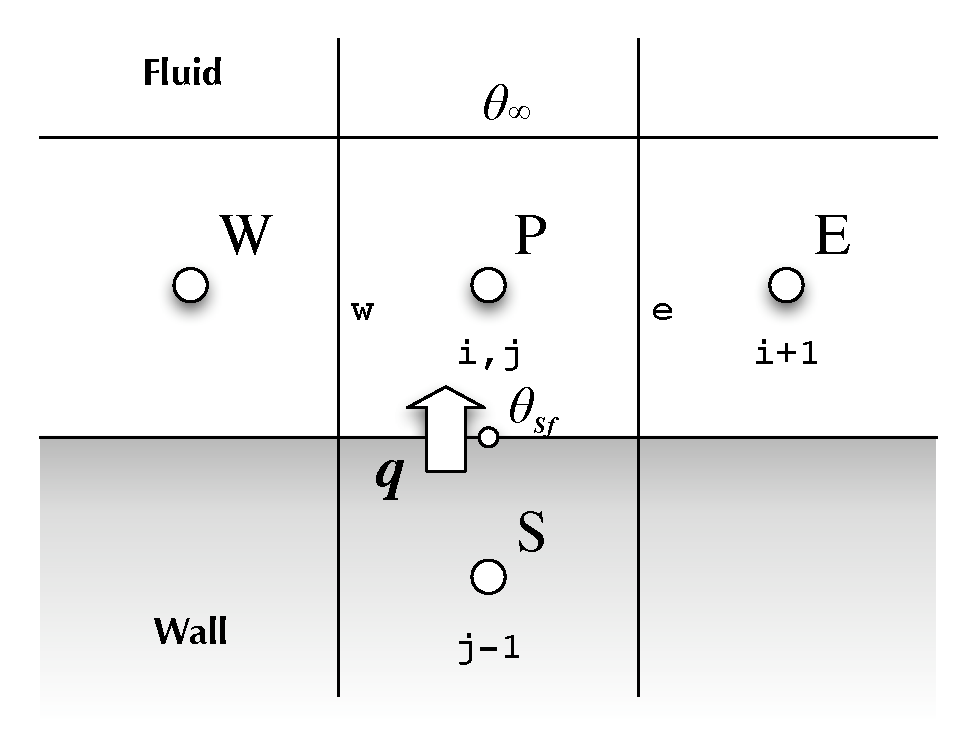
\includegraphics[width=6cm,clip]{HeatTransfer.eps}
\caption{固体壁面での熱伝達}
\label{fig:heat transfer on solid}
\end{center}
\end{figure}

指定面における熱伝達境界条件の実装方法として,次の3つの場合が考えられる.
\begin{indentation}{3zw}{0zw}
\begin{description}
\item[タイプ N)] 熱伝達係数を与え,計算結果の固体表面温度から熱流束を計算する.共役熱移動の場合に利用する.
\item[タイプ S)] 表面温度と熱伝達係数を与え,熱流束を計算する.流体のみを解く場合に利用する.
\item[タイプ B)] 熱伝達係数とバルク温度を与え,熱流束を計算する.固体の熱移動のみを解く場合の境界条件として利用する.
\item[タイプ SNB/SNL)] 自然対流の乱流熱伝達の実験式を実装したもの.流体のみを解く場合に利用し,タイプSを拡張している.SNBは温度差の定義にバルク温度を用い,SNLは隣接セルの値を用いた実装である.
\item[タイプ SFB/SFL)] 強制対流の層流・乱流熱伝達の実験式を実装したもの.流体のみを解く場合に利用し,タイプSを拡張している.SFBは温度差の定義にバルク温度を用い,SFLは隣接セルの値を用いた実装である.
\end{description}
\end{indentation}

%
\paragraph{Nusselt数とStanton数}
まず,ヌセルト数との関連を示す.ヌセルト数の定義は,熱伝導に対する熱伝達の比なので,

\begin{equation}
Nu \,=\, \frac{HL^{\prime}}{\lambda}, \qquad \left.
\begin{array}{ll}
H & [W/(m^2K)]\\
\lambda & [W/(mK)]\\
L^\prime & [m]
\end{array} \right\}
\label{eq:nu_1}
\end{equation}

フーリエの法則とニュートンの冷却則から,

\begin{equation}
{H} \,=\, \lambda {\left({\frac{\mathrm{\partial}{\mathit{\theta}}'}{\mathrm{\partial}{n}'}}\right)}_{{n}'\mathrm{{=}}{0}}\, \Bigg/ {\mathrm{\Delta}{\mathit{\theta}}'}
\,=\,
\frac{{\mathit{\lambda}}\mathrm{\Delta}{\mathit{\theta}}'}{{L}'\mathrm{\Delta}{\mathit{\theta}}'}{\left({\frac{\mathrm{\partial}\mathit{\theta}}{\mathrm{\partial}{n}}}\right)}_{{n}\mathrm{{=}}{0}}
\,=\,
\frac{{\mathit{\lambda}}}{{L}'}{\left({\frac{\mathrm{\partial}\mathit{\theta}}{\mathrm{\partial}{n}}}\right)}_{{n}\mathrm{{=}}{0}}
\label{eq:nu_2}
\end{equation}

\begin{equation}
Nu \,=\, \left( \frac{\partial \theta}{\partial n} \right)_{n=0}
\label{eq:nu_3}
\end{equation}

一方,熱流束を表す\textbf{式(\ref{eq:pscalar qbc})}の無次元形式は,\textbf{式(\ref{eq:qD})}となり,これはStanton数を表す.つまり,

\begin{equation}
q \,=\, \frac{q^\prime}{u_{\mathit 0}^\prime \Delta \theta^\prime} \frac{1}{\rho^\prime C}
\quad \equiv \quad 
St\,=\, \frac{Nu}{Re Pr} 
\label{eq:stanton}
\end{equation}


%
\paragraph{タイプ N}
タイプNの計算は固体表面セルの温度は計算によって決まる値を用い,熱伝達係数($H>0$)のみで計算できる.\textbf{図\ref{fig:typeN}}には,固体と流体の相対的な位置が異なる(a), (b)2つのパターンを示している.いま,セル境界において,正の熱流束$q_{j+1/2}^{\prime}>0$を仮定する.つまり,

\begin{equation}
q_{j+1/2}^{\prime}\,=\,-H(\theta_{j+1}^{\prime}-\theta_{j}^{\prime})\, >\,0 \quad \Longleftrightarrow \quad \theta_{j}^{\prime} \,>\, \theta_{j+1}^{\prime}
\label{eq:qT_N1}
\end{equation}

$q_{j+1/2}^{\prime}>0$なので,jセルは冷却, j+1セルは加熱となる.次に,セル界面において負の熱流束$q_{j+1/2}^{\prime}<0$を仮定すると,

\begin{equation}
q_{j+1/2}^{\prime} \,=\,-H(\theta_{j+1}^{\prime}-\theta_{j}^{\prime})\, <\,0 \quad \Longleftrightarrow \quad \theta_{j}^{\prime} \,<\, \theta_{j+1}^{\prime}
\label{eq:qT_N2}
\end{equation}

したがって,熱伝達形式の境界熱流束$q_{T}'$は,常に次式で計算できる.

\begin{equation}
q_{T,\,j+1/2}^{\prime} \,=\,-H(\theta_{j+1}^{\prime}-\theta_{j}^{\prime})
\label{eq:qT_N3}
\end{equation}

\textbf{式(\ref{eq:qbc non-dimansionalize})}を用いて無次元化すると,

\begin{equation}
q_{T,\,j+1/2} \,=\, - \frac{1}{\rho^{\prime} C} \frac{H}{{u_{\mathit{0}}}^{\prime}}(\theta_{j+1}-\theta_{j})
\label{eq:qT_N4}
\end{equation}

ここで$\rho^{\prime}C$は,単媒質の場合には代表媒質の物性値である.

\begin{figure}[htdp]
\begin{center}
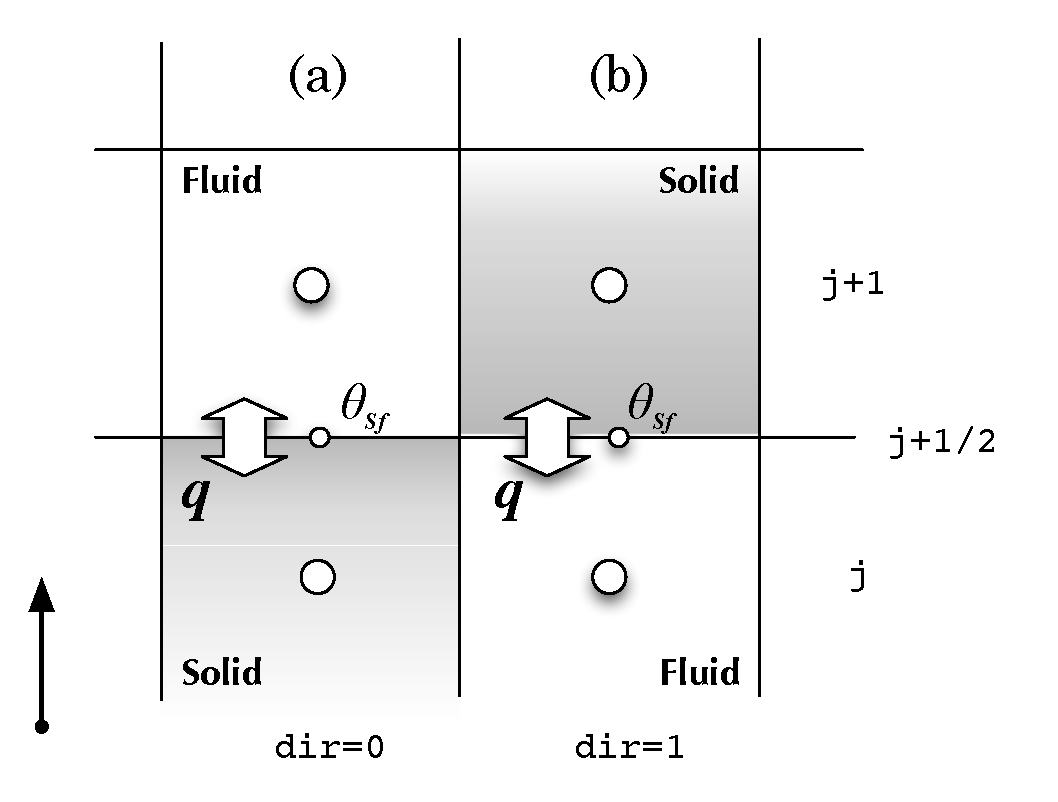
\includegraphics[width=7cm,clip]{typeN.eps}
\caption{熱伝達境界タイプN/Sのパターン.方向フラグdirは\textbf{式(\ref{eq:qT_S1})}で用いるインデクスjに対する相対的な位置を示す.}
\label{fig:typeN}
\end{center}
\end{figure}

\begin{indentation}{3zw}{0zw}
{
\small
\begin{program}
<Elem name="Heat_Transfer_N" id="68"  comment="HF_1">
  <Param name="def_face"    dtype="INT"    value="1" />
  <Param name="Coef_of_Heat_Transfer" dtype="REAL" value="1.2e-2"/>
</Elem>
\end{program}
}
\end{indentation}

%
\paragraph{タイプ S}
この境界条件は想定する表面温度と熱伝達係数を与える.熱流体計算で固体側を解かず,流体のみを解く場合の境界条件として用いる.
\textbf{図\ref{fig:typeN}}を参照して,参照温度を外側1点目にとる場合,パターン(a)の$dir=0$のときに法線が正になるようにインデクス計算を行うと,

\begin{equation}
q_{T,\,j+1/2} \,=\, - \frac{1}{\rho^{\prime}C} \frac{H}{{u_{\mathit{0}}}^{\prime}} \left( \theta_{j+1-dir} -\theta_{sf} \right) \left( 1-2{dir} \right)
\label{eq:qT_S1}
\end{equation}

\noindent また,参照温度を基準温度にとる場合,
\begin{equation}
q_{T,\,j+1/2} \,=\, - \frac{1}{\rho^{\prime}C} \frac{H}{{u_{\mathit{0}}}^{\prime}} \left( \theta_0 -\theta_{sf} \right) \left( 1-2{dir} \right)
\label{eq:qT_S1_2}
\end{equation}

\noindent タイプSの実装は,\textbf{式(\ref{eq:qT_S1_2})}である.

次の例では,ID=67に80度の温度が与えられ,ID=1と挟まれる面に熱伝達係数$H=0.012\, [W/(m^{2}K)]$が与えられる.

\begin{indentation}{3zw}{0zw}
{
\small
\begin{program}
<Elem name="Heat_Transfer_S" id="67"  comment="HF_2">
  <Param name="def_face"    dtype="INT"    value="1" />
  <Param name="Surface_Temperature" dtype="REAL" value="80.0"/>
  <Param name="Coef_of_Heat_Transfer" dtype="REAL" value="1.2e-2"/>
</Elem>
\end{program}
}
\end{indentation}

%
\paragraph{タイプ B}
この境界条件は固体熱伝導を解く場合の境界条件である.つまり,固体セルのみを解き,流体セルは解かない場合に用い,流体の参照温度と熱伝達係数を指定する.計算式は\textbf{式(\ref{eq:qT_B1})}を用いる.参照する流体のインデクスは,\textbf{図\ref{fig:typeB}}のように,タイプN/S と参照方向が逆になっている.パターン(a)の場合に熱伝達面からの法線は正,(b)の場合に法線が負になるように,方向を表すインデクス計算を$2dir-1$として,

\begin{equation}
q_{T,\,j+1/2} \,=\, \frac{1}{\rho^{\prime}C} \frac{H}{{u_{\mathit{0}}}^{\prime}} \left( \theta_{j+1-dir} -\theta_{\infty} \right) \left( 2{dir} -1\right)
\label{eq:qT_B1}
\end{equation}

次の例では,ID=60に10度の温度が与えられ,ID=1と挟まれる面に熱伝達係数$H=0.2\, [W/(m^{2}K)]$が与えられる.

\begin{indentation}{3zw}{0zw}
{
\small
\begin{program}
<Elem name="Heat_Transfer_B" id="60"  comment="HF_3">
  <Param name="def_face"    dtype="INT"    value="1" />
  <Param name="Bulk_Temperature" dtype="REAL" value="10.0"/>
  <Param name="Coef_of_Heat_Transfer" dtype="REAL" value="0.2"/>
</Elem>
\end{program}
}
\end{indentation}

\begin{figure}[htdp]
\begin{center}
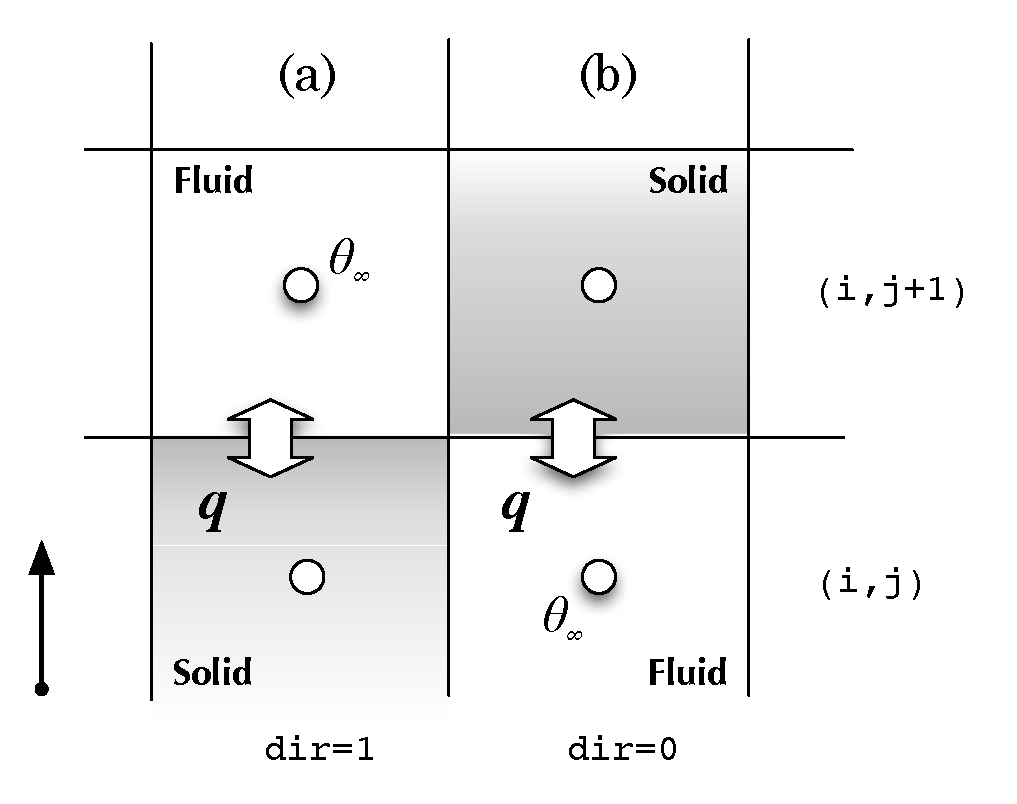
\includegraphics[width=7cm,clip]{typeB.eps}
\caption{熱伝達境界Bのパターン.}
\label{fig:typeB}
\end{center}
\end{figure}



%
\paragraph{タイプ SNB/SNL}
文献\cite{shouji:95:Dennetsu}には,平板に対する自然対流の層流と乱流の熱伝達に関する近似式が説明されている.雰囲気流体の温度に比べ加熱面の温度が非常に高い場合,平板が長くなると境界層が不安定になり,ほぼ$Ra>10^9$で層流から乱流へ遷移する.垂直平板に関する平均熱伝達$(\overline{Nu_L},代表長L)$は次式で整理される.

\begin{equation}
\left.
\begin{array}{lll}
\vspace{1mm}
層流 & \overline{Nu_L} \,=\, 0.59Ra_L^{1/4} & (10^4 < Ra_L < 10^9)\\
乱流 & \overline{Nu_L} \,=\, 0.10Ra_L^{1/3} & (10^9 < Ra_L < 10^{13})
\end{array} \right\}
\label{eq:natural_convection_vert_ht}
\end{equation}

一方,水平平板の場合には,加熱面が上面と下面にある場合で雰囲気流体の挙動が異なるため,\textbf{式(\ref{eq:natural_convection_horiz_ht})}のように整理されている.

\begin{equation}
\left.
\begin{array}{lll}
\vspace{1mm}
上面加熱 & \overline{Nu_L} \,=\, 0.54Ra_L^{1/4} & (10^4 < Ra_L < 10^7)\\
\vspace{1mm}
上面加熱 & \overline{Nu_L} \,=\, 0.15Ra_L^{1/3} & (10^7 < Ra_L < 10^{11})\\
\vspace{1mm}
下面加熱 & \overline{Nu_L} \,=\, 0.27Ra_L^{1/4} & (10^5 < Ra_L < 10^{10})
\end{array} \right\}
\label{eq:natural_convection_horiz_ht}
\end{equation}

\noindent 上記の自然対流熱伝達の整理式を\textbf{図\ref{fig:natural_heat_transfer}}に示す.\\

\begin{figure}[htdp]
\begin{center}
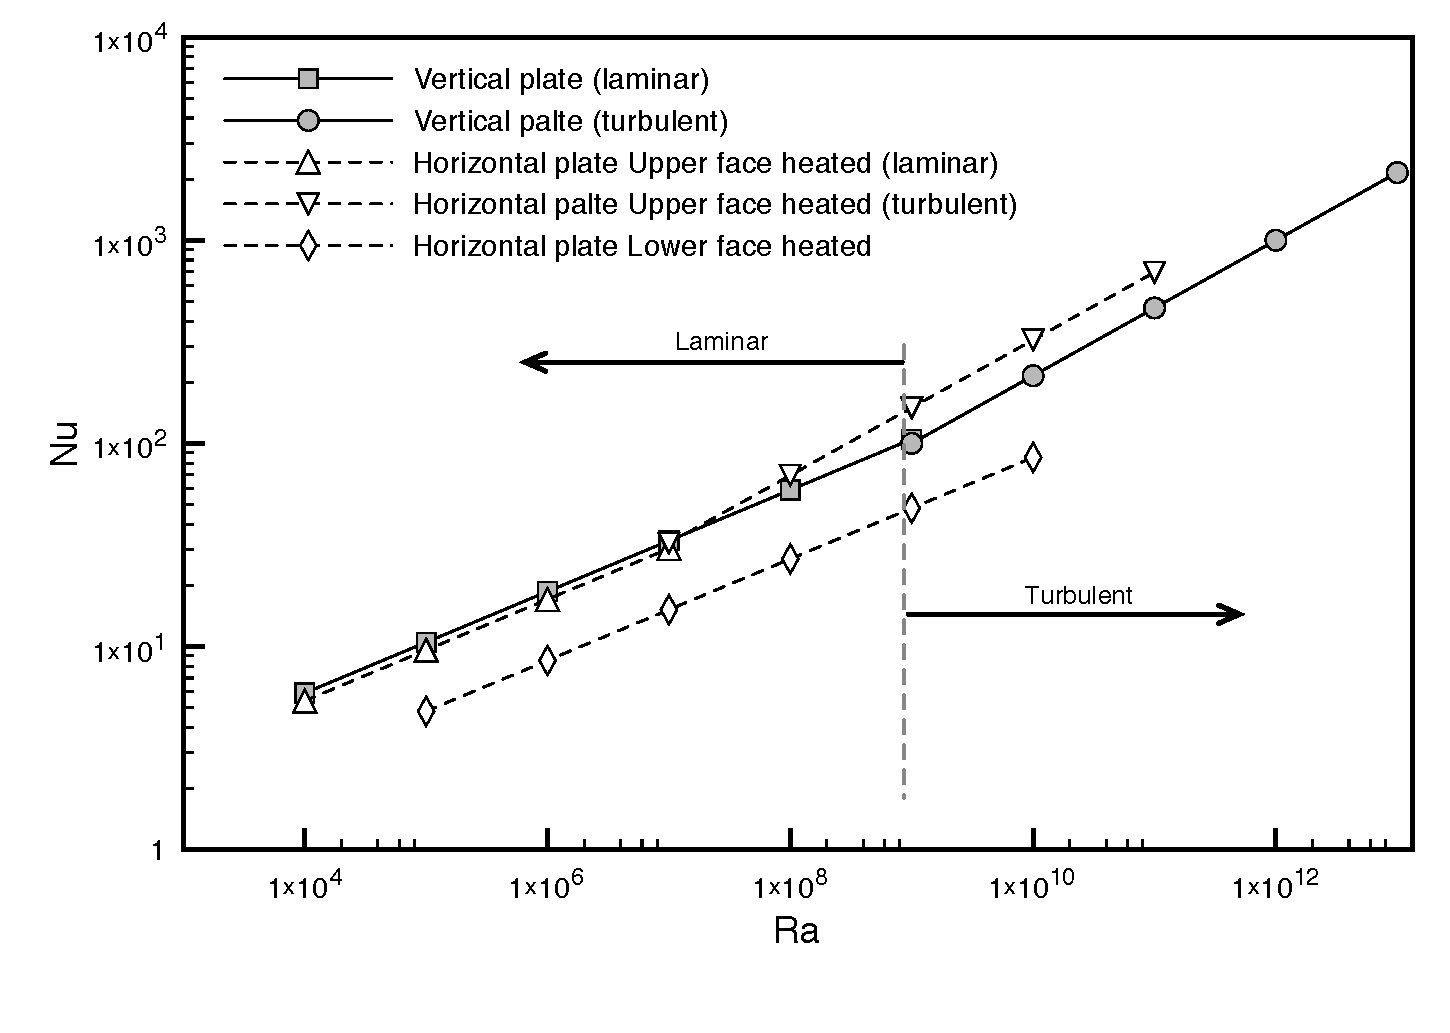
\includegraphics[width=12cm,clip]{HeatTransfer_Natural.eps}
\caption{自然対流熱伝達の整理式\cite{shouji:95:Dennetsu}}
\label{fig:natural_heat_transfer}
\end{center}
\end{figure}

これらの整理式を見ると,大まかには垂直面の実験式を用いて水平面の上面を近似できると考える.そこで,水平面の上面と垂直面,水平面の下面の2つのパターンについて,層流と乱流の実験式を用いることにする.境界条件のパラメータで与える値を\textbf{表\ref{tbl:heat transfer type SN para}}に示す.標準的には,\textbf{式(\ref{eq:natural_convection_vert_ht})}, \textbf{式(\ref{eq:natural_convection_horiz_ht})}の値を用いる.

\begin{table}[htdp]
\caption{自然対流熱伝達のパラメータ}
\begin{center}
\small
\begin{tabular}{ll}\toprule
パラメータタグ & 記号の意味\\ \midrule
vertival\_laminar\_alpha & 垂直平板の層流時の係数$\alpha$\\
vertival\_laminar\_beta & 垂直平板の層流時の係数$\beta$\\
vertival\_turbulent\_alpha & 垂直平板の乱流時の係数$\alpha$\\
vertival\_turbulent\_beta & 垂直平板の乱流時の係数$\beta$\\
vertival\_Ra\_critial & 垂直平板の臨界Ra数$Ra_L$\\
lower\_laminar\_alpha & 水平平板(下面)の層流時の係数$\alpha$\\
lower\_laminar\_beta & 水平平板(下面)の層流時の係数$\beta$\\
lower\_turbulent\_alpha & 水平平板(下面)の乱流時の係数$\alpha$\\
lower\_turbulent\_beta & 水平平板(下面)の乱流時の係数$\beta$\\
lower\_Ra\_critial & 水平平板(下面)の臨界Ra数$Ra_L$\\ 
type & BULK\_TEMPERATURE or LOCAL\_TEMPERATURE\\ \bottomrule
\end{tabular}
\end{center}
\label{tbl:heat transfer type SN para}
\end{table}

次に,タイプSNの熱伝達境界条件の実装について説明する.\textbf{式(\ref{eq:natural_convection_vert_ht})},\textbf{式(\ref{eq:natural_convection_horiz_ht})}は形式的に次式のように表せる.

\begin{equation}
\overline{Nu_L} \,=\, \alpha {Ra_L}^{\,\beta}
\label{eq:typeSN_form}
\end{equation}

\noindent \textbf{式(\ref{eq:nu_1})}と\textbf{式(\ref{eq:typeSN_form})}から,

\begin{equation}
H \,=\, \alpha Ra_L^\beta \frac{\lambda}{L^\prime}
\label{eq:typeSN_form_ht}
\end{equation}

\noindent \textbf{式(\ref{eq:qT2})}と\textbf{式(\ref{eq:qbc non-dimansionalize})}から,

\begin{equation}
q \,=\, - \frac{q^\prime}{{u_\mathit{0}}^\prime \Delta \theta^\prime \rho^\prime C}
\,=\, - \frac{H (\theta_{sf}\,-\,\theta_\infty)}{{u_\mathit{0}}^\prime \rho^\prime C}
\,=\, - \frac{\lambda (\theta_{sf}\,-\,\theta_\infty)}{{u_\mathit{0}}^\prime L^\prime \rho^\prime C} \, \alpha Ra_L^\beta
\label{eq:typeSN_heat_flux}
\end{equation}

\noindent ここで,水平面の上下面では熱伝達が大きく異なるので,z軸方向が重力方向と仮定して,上下面で選択的な実装を行う.上下面の選択は\textbf{図\ref{fig:typeN}}から,

\begin{equation}
\left.
\begin{array}{ll}
\vspace{1mm}
上面加熱 & dir=0\\
\vspace{1mm}
下面加熱 & dir=1
\end{array} \right\}
\label{eq:selection of face}
\end{equation}

\subparagraph{SNL}
\noindent 参照点をひとつ外側の点にとるタイプSNLの場合,パラメータにLOCAL\_TEMPERATUREを指定する.
\textbf{式(\ref{eq:selection of face})}の関係を用いて,\textbf{式(\ref{eq:qT_S1})}に倣い,

\begin{equation}
q_{T,\,j+1/2} \,=\, - \frac{\lambda \left( \theta_{j+1-dir} -\theta_{sf} \right)}{{u_\mathit{0}}^\prime L^\prime \rho^\prime C} \, \alpha Ra_L^\beta \, \left( 1-2{dir} \right)
\label{eq:typeSN_heat_flux_ND}
\end{equation}

\subparagraph{SNB}
参照点を基準温度(BaseTmp)にとるSNBの場合,BULK\_TEMPERATUREを指定する.

\begin{equation}
q_{T,\,j+1/2} \,=\, - \frac{\lambda \left( \theta_0 -\theta_{sf} \right)}{{u_\mathit{0}}^\prime L^\prime \rho^\prime C} \, \alpha Ra_L^\beta \, \left( 1-2{dir} \right)
\label{eq:typeSN_heat_flux_ND_2}
\end{equation}


次の例では,ID=67に80度の温度が与えられ,ID=1と挟まれる面に\textbf{式(\ref{eq:natural_convection_vert_ht})},\textbf{(\ref{eq:natural_convection_horiz_ht})}の熱伝達係数が与えられる.

\begin{indentation}{3zw}{0zw}
\small
\begin{program}
<Elem name="Heat_Transfer_SN" id="67"  comment="HF_2">
  <Param name="def_face"    dtype="INT"    value="1" />
  <Param name="type"    dtype="STRING"    value="BULK_TEMPERATURE" />
  <Param name="Surface_Temperature" dtype="REAL" value="80.0"/>
  <Param name="vertival_laminar_alpha" dtype="REAL" value="0.59"/>
  <Param name="vertival_laminar_beta"  dtype="REAL" value="0.25"/>
  <Param name="vertival_turbulent_alpha" dtype="REAL" value="0.1"/>
  <Param name="vertival_turbulent_beta"  dtype="REAL" value="0.3333333"/>
  <Param name="vertival_ra_critial" dtype="REAL" value="1.0e9"/>
  <Param name="lower_laminar_alpha" dtype="REAL" value="0.27"/>
  <Param name="lower_laminar_beta"  dtype="REAL" value="0.25"/>
  <Param name="lower_turbulent_alpha" dtype="REAL" value="0.27"/>
  <Param name="lower_turbulent_beta"  dtype="REAL" value="0.25"/>
  <Param name="lower_ra_critial" dtype="REAL" value="1.0e9"/>
</Elem>
\end{program}
\end{indentation}

%
\paragraph{タイプ SFB/SFL}
強制対流熱伝達の実験式を組み込んだ熱伝達境界条件を与える.
文献\cite{shouji:95:Dennetsu}から,平板に対する発達した強制対流の乱流熱伝達は,実験による摩擦係数の測定結果とチルトン-コルバーンのアナロジーを用い,温度一定で平板が遷移長さよりも十分に大きいと仮定すると,\textbf{式(\ref{eq:forced_convection_ht})}のように表せる.\textbf{図\ref{fig:forced_heat_transfer}}には幾つかの$Pr$数に対する熱伝達の様子を示す.

\begin{equation}
\overline{Nu_L} \,=\, 0.037Re_L^{4/5}Pr^{1/3}
\label{eq:forced_convection_ht}
\end{equation}

\begin{figure}[htdp]
\begin{center}
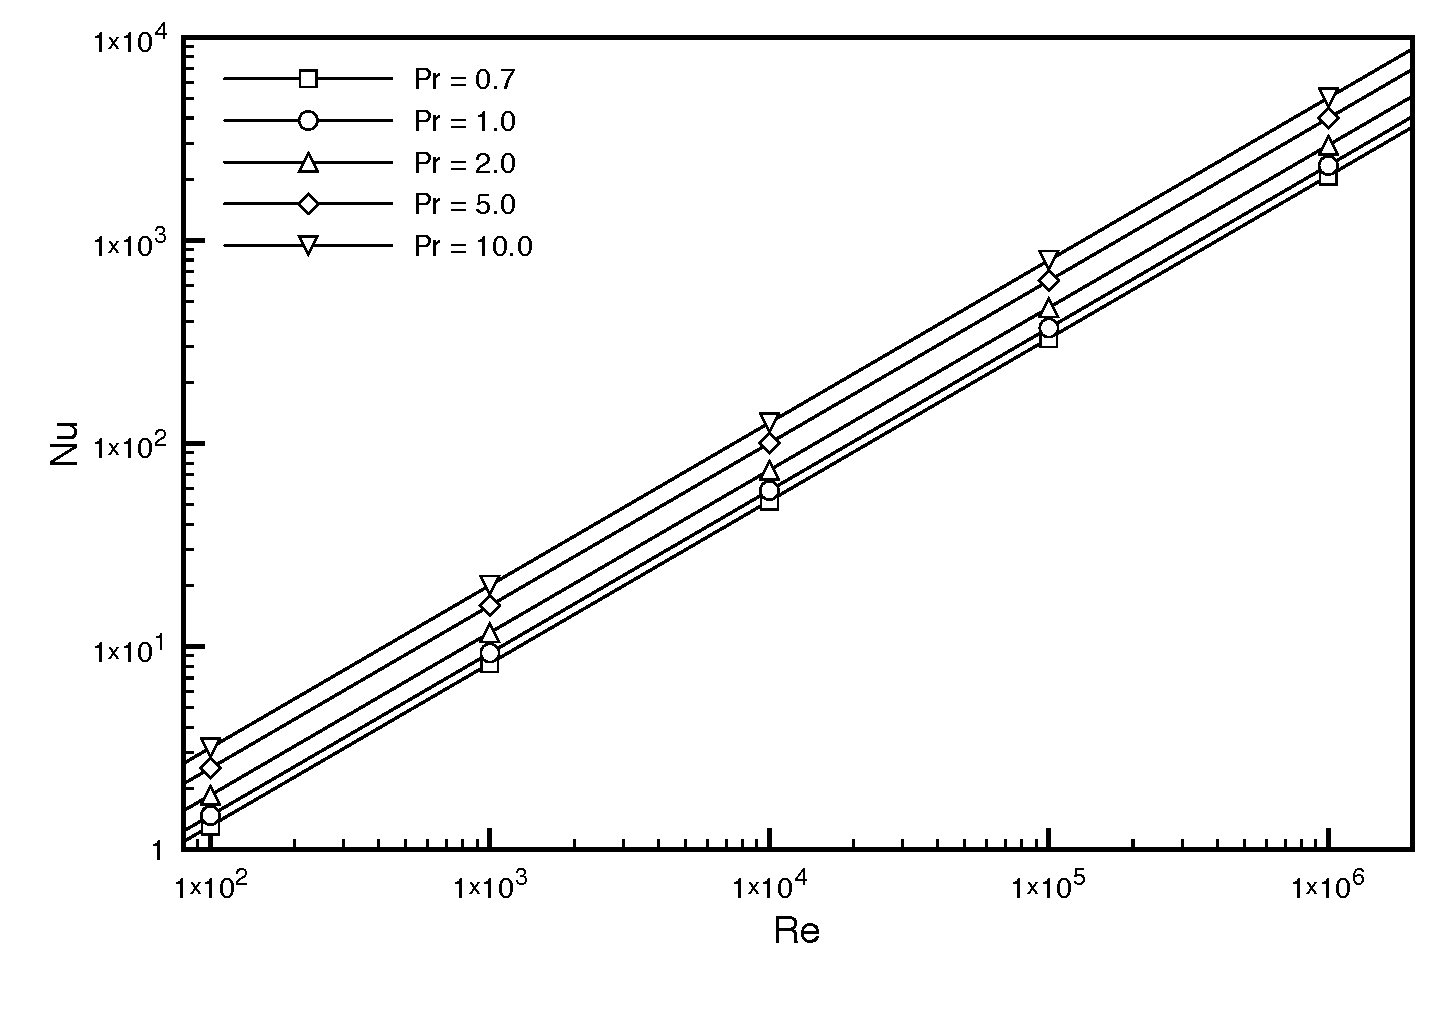
\includegraphics[width=12cm,clip]{HeatTransfer_Forced.eps}
\caption{強制対流熱伝達\cite{shouji:95:Dennetsu}}
\label{fig:forced_heat_transfer}
\end{center}
\end{figure}

\noindent 熱伝達係数の形式を次のように表し,タイプSNと同様に書き下すと,

\begin{equation}
H \,=\, \alpha Re_L^\beta \, Pr^\gamma \, \frac{\lambda}{L^\prime}
\label{eq:typeSF_form_ht}
\end{equation}

タイプSNと同様に,\textbf{式(\ref{eq:typeSF_form_ht})}のパラメータを\textbf{表\ref{tbl:heat transfer type SF para}}で与える.

\begin{table}[htdp]
\caption{強制対流熱伝達のパラメータ}
\begin{center}
\small
\begin{tabular}{ll}\toprule
パラメータタグ & 記号の意味\\ \midrule
alpha & 係数$\alpha$\\
beta & 係数$\beta$\\
gamma & 係数$\gamma$\\
type & BULK\_TEMPERATURE or LOCAL\_TEMPERATURE\\ \bottomrule
\end{tabular}
\end{center}
\label{tbl:heat transfer type SF para}
\end{table}

次に,タイプSFの熱伝達境界条件の実装について説明する.\textbf{式(\ref{eq:typeSF_form_ht})}は温度差の取り方により,次の2つのタイプがある.

\subparagraph{SFL}
参照点を一つ外側にとる場合,パラメータにLOCAL\_TEMPERATUREを指定する.
\begin{equation}
q_{T,\,j+1/2} \,=\, - \frac{\lambda \left( \theta_{j+1-dir} -\theta_{sf} \right)}{{u_\mathit{0}}^\prime L^\prime \rho^\prime C} \, \alpha Re_L^\beta \, Pr^\gamma \,\left( 1-2{dir} \right)
\label{eq:typeSF_heat_flux_ND}
\end{equation}

\subparagraph{SFB}
参照点を基準温度(BaseTmp)にとるSFBの場合,BULK\_TEMPERATUREを指定する.
\begin{equation}
q_{T,\,j+1/2} \,=\, - \frac{\lambda \left( \theta_0 -\theta_{sf} \right)}{{u_\mathit{0}}^\prime L^\prime \rho^\prime C} \, \alpha Re_L^\beta \, Pr^\gamma \,\left( 1-2{dir} \right)
\label{eq:typeSF_heat_flux_ND_2}
\end{equation}


次の例では,ID=60に80度の温度が与えられ,ID=1と挟まれる面に\textbf{式(\ref{eq:forced_convection_ht})}の熱伝達係数が与えられる.

\begin{indentation}{3zw}{0zw}
\small
\begin{program}
<Elem name="Heat_Transfer_SF" id="60"  comment="HF_3">
  <Param name="def_face"    dtype="INT"    value="1" />
  <Param name="type"    dtype="STRING"    value="LOCAL_TEMPERATURE" />
  <Param name="Surface_Temperature" dtype="REAL" value="80.0"/>
  <Param name="alpha" dtype="REAL" value="0.037"/>
  <Param name="beta"  dtype="REAL" value="0.8"/>
  <Param name="gamma" dtype="REAL" value="0.333333"/>
</Elem>
\end{program}
\end{indentation}


%
\subsubsection{等温境界 $q_{ISO}$}
指定面で温度が一定となる境界条件で,面温度を一定に保つような熱流束が発生する.ここで扱う等温境界は,固体−流体界面と固体−固体界面の2つの場合が考えられる.境界面は,IsoThermalのIDとdef\_faceにより挟まれる面となる.

\begin{figure}[htdp]
\begin{center}
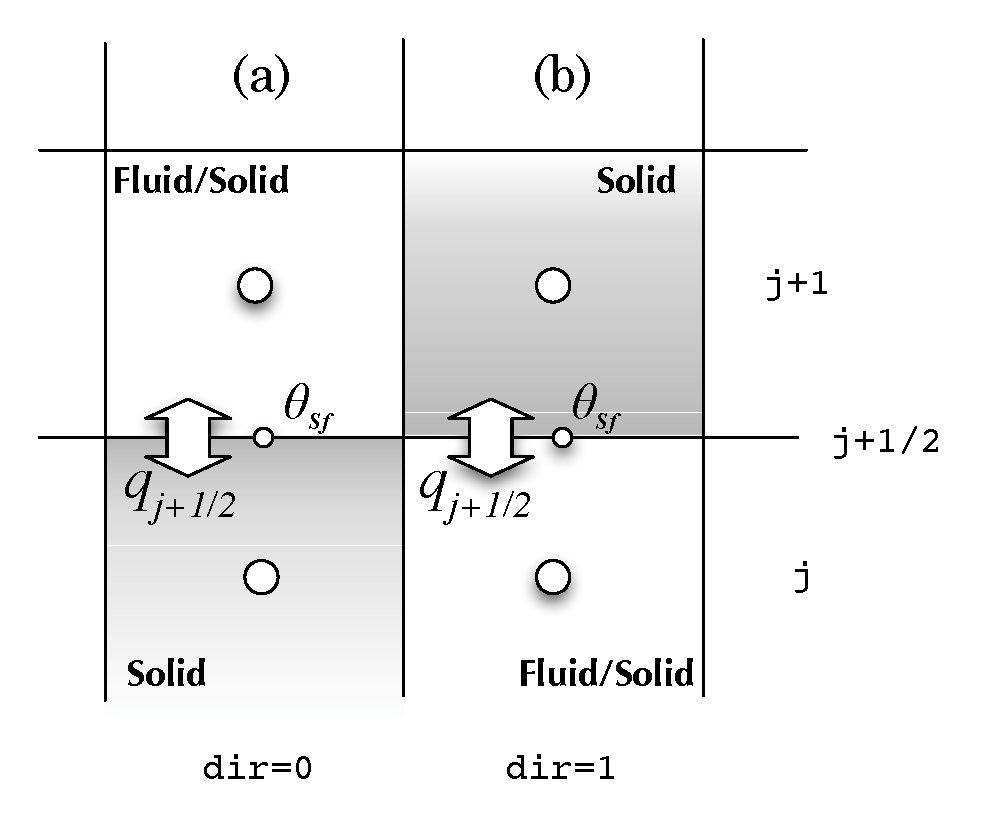
\includegraphics[width=7cm,clip]{Isothermal.eps}
\caption{等温境界のパターン.方向フラグdirはIsoThermalセルの位置と法線方向を示す.}
\label{fig:iso-thermal}
\end{center}
\end{figure}

\noindent \textbf{図\ref{fig:iso-thermal}}において,色塗りのSolidセルは IsoThermalのIDがつけられたセルである.(a), (b) の各パターンはIsoThermalセルの位置が異なる.dir は前処理段階で設定される方向インデクスである.(a) の場合は,界面と温度指定のSolidセルのインデクスが両方とも j であるので,dir=0 とする.このとき,IsoThermalセルからの法線方向は正である.一方,(b) の場合は,界面インデクスはjであるが,等温指定のSolidセルは j+1 なので,dir=1 とする.このとき,IsoThermalセルからの法線方向は負である.

(a)のパターン(dir=0)を考える.セル j は固体セルで,表面温度は常に指定温度である.計算する方のセル j+1 側からの熱流束を考えると,片側近似により,

\begin{equation}
{{q}'}_{{ISO}{\mathrm{,}}\hspace{0.33em}{j}\mathrm{{+}}{1}{\mathrm{/}}{2}}\mathrm{{=}}\mathrm{{-}}{{\mathit{\lambda}}}_{{j}\mathrm{{+}}{1}}\frac{{{\mathit{\theta}}'}_{{j}\mathrm{{+}}{1}}\mathrm{{-}}{{\mathit{\theta}}'}_{sf}}{{{h}'}\slash{2}}
\label{eq:qiso1}
\end{equation}

\noindent 無次元化すると,

\begin{equation}
q_{ISO,\hspace{0.3em}j+1/2} 
\sim
\frac{q_{ISO}^{\prime}}{u_{\mathit{0}}^{\prime} \Delta \theta^{\prime}} \frac{1}{\rho^{\prime}C}
\,=\,
- \frac{1}{u_{\mathit{0}}^{\prime} \Delta \theta^{\prime}} \frac{\lambda_{j+1}}{\rho^{\prime}C}\frac{\theta_{j+1}^{\prime} - \theta_{sf}^{\prime}}{h^{\prime}\slash{2}}
\,=\,
- \frac{2}{u_{\mathit{0}}^{\prime} L^{\prime}} \frac{\lambda_{j+1}}{\rho^{\prime}C} \frac{\theta_{j+1} - \theta_{sf}}{h}
\label{eq:qiso2-1}
\end{equation}

一方,(b)のパターン(dir=1)は,セル j+1 は固体セルで常に指定温度である.

\begin{equation}
{{q}'}_{{ISO}{\mathrm{,}}\hspace{0.33em}{j}\mathrm{{+}}{1}{\mathrm{/}}{2}}\mathrm{{=}}\mathrm{{-}}{{\mathit{\lambda}}}_{j}\frac{{{\mathit{\theta}}'}_{sf}\mathrm{{-}}{{\mathit{\theta}}'}_{j}}{{{h}'}\slash{2}}
\label{eq:qiso2}
\end{equation}

\begin{equation}
q_{ISO,\hspace{0.3em}j+1/2} 
\sim
\frac{q_{ISO}^{\prime}}{u_{\mathit{0}}^{\prime} \Delta \theta^{\prime}} \frac{1}{\rho^{\prime}C}
\,=\,
- \frac{1}{u_{\mathit{0}}^{\prime} \Delta \theta^{\prime}} \frac{\lambda_{j}}{\rho^{\prime}C}\frac{\theta_{sf}^{\prime} - \theta_{j}^{\prime}}{h^{\prime}\slash{2}}
\,=\, - \frac{2}{u_{\mathit{0}}^{\prime} L^{\prime}} \frac{\lambda_{j}}{\rho^{\prime}C}\frac{\theta_{sf} -\theta_{j}}{h}
\label{eq:qiso3}
\end{equation}

\noindent 計算する流体または固体セルは$j+1-dir$で表されること,基準セルに注意してパターン(a), (b) をまとめると,単媒質の場合,

\begin{equation}
q_{ISO,\hspace{0.3em}j+1/2} 
\,=\,
- \frac{2}{u_{\mathit{0}}^{\prime} L^{\prime}} \frac{\lambda_{j+1-dir}}{\rho^{\prime}C}\frac{\theta_{j+1-dir}-\theta_{sf}}{h} \left( 1-2dir \right)
\label{eq:qiso4}
\end{equation}

\noindent ここで$1-2dir$はパターン(a)のとき,つまり$dir=0$のときに法線が正になるように構成している.\\

次の例では,ID=70とID=1に挟まれる面を30度の等温面として扱うことを指定している.

\begin{indentation}{3zw}{0zw}
{
\small
\begin{program}
<Elem name="Iso_Thermal" id="70"  comment="iso_1">
  <Param name="def_face"    dtype="INT"    value="1" />
  <Param name="Temperature" dtype="REAL" value="30.0"/>
</Elem>
\end{program}
}
\end{indentation}

%
\subsubsection{輻射境界 $q_R$}
熱輻射の計算を行う場合に用いる.輻射境界条件は,形態係数の計算を行い輻射流束の収支計算を行った後,その熱流束を直接熱流束境界として与える.

\begin{indentation}{3zw}{0zw}
{
\small
\begin{program}
<Elem name="Heat_Face" id="0">
  <Elem name="Radiation" id="75"  comment="rad_1">
    <Param name="def_face"    dtype="INT"    value="1" />
    <Param name="epsilon" dtype="REAL" value="0.2"/>
    <Param name="projection" dtype="REAL" value="0.6"/>
  </Elem>
</Elem>
\end{program}
}
\end{indentation}

%
\subsubsection{断熱境界 $q_A$}
断熱境界$q_A$は空間におけるセル数の出現頻度が多くなることが予想されるため,他の境界条件とは異なり,断熱マスクにより離散式中に組み込んでいる.このため,モデル作成時にIDで指定することになる.
断熱面の境界条件は,Adiabatic の指定により導入する.
Adiabaticの指定は,idとdef\_faceで指定される面を断熱境界と解釈する.下記の例では,ID=40とID=1で挟まれる面が断熱面となる.

{
\small
\begin{program}
<Elem name="Adiabatic" id="40" comment="insulation">
  <Param name="def_face"    dtype="INT"    value="1" />
</Elem>
\end{program}
}

\begin{figure}[htdp]
\begin{center}
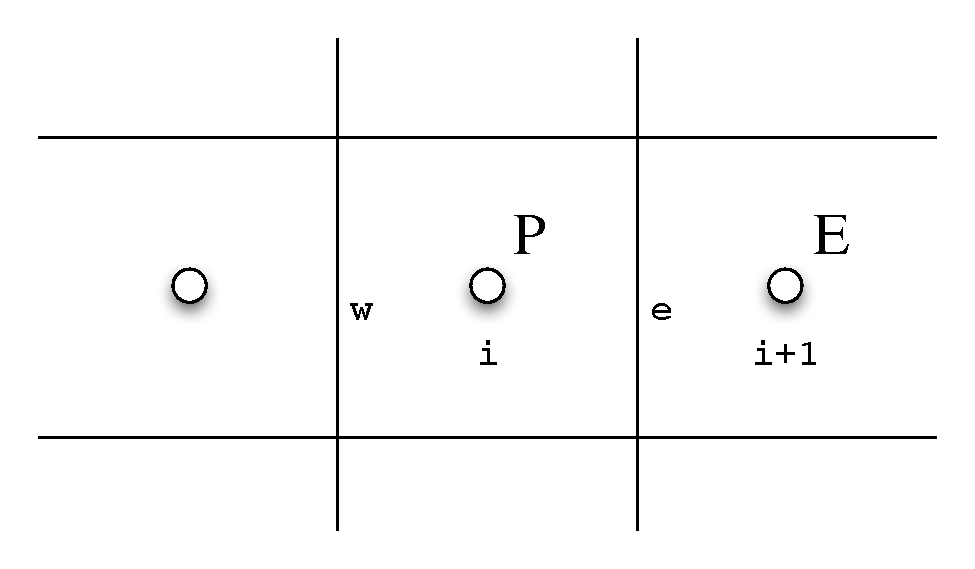
\includegraphics[width=7cm,clip]{AdiabaticBC.eps}
\caption{セルインデックスとセル界面の指定}
\label{fig:face definition}
\end{center}
\end{figure}

\textbf{図\ref{fig:face definition}}において,$e$面($i+1/2$ 位置のセル面)が断熱面の場合,断熱フラグはセル要素に対してスタガード変数配置と同じインデクスで表す.今,$i$ 方向の $e$ 面が断熱面とすると,\textbf{図\ref{fig:BCIndex}}のBC Index の18ビット目を0にして,BCの情報をエンコードする.
断熱条件は,断熱マスク式(\ref{eq:gamma A definition})により実装される.


%
\subsection{セルボリュームに対する熱境界条件の実装}
\label{sec:volume heat bc}
%
\subsubsection{発熱源}
発熱・吸熱の境界条件は,セルボリュームに対して与える.単位体積あたりの発熱量$Q^\prime \,[W/m^3]$が与えられると,発熱項は\textbf{式(\ref{eq:passive scalar1-2 ND})}により無次元化される.ボクセルモデルのIDに対して,XMLファイルで熱源を発熱量(heat release value)または発熱密度(heat generation density)により指定する.この例では,ID=246 に対して,10.0 $[W/m^3]$ の発熱密度を与えている.
{
\small
\begin{program}
<Elem name="Heat_Volume" id="1">
  <Elem name="Heat_Generation" id="246" comment="Desktop">
    <Param name="heat_generation_density" dtype="REAL" value="10.0"/>
  </Elem>
</Elem>
\end{program}
}

熱源項は,安定性のため一時刻前の値を用いて線形化する.ここで注意すべき点は,発熱源の媒質の物性値の指定である(\textbf{式(\ref{eq:qV2})}中の$\rho^{\prime},\,C$)).単媒質の場合には,指定された媒質の物性値を用いる.現物が複数の媒質から構成されている場合には適切な物性値を推定する必要がある.

\begin{equation}
{\mathit{\theta}}^{\hspace{0.15em}n+1}\,=\,{\mathit{\theta}}^{\hspace{0.15em}n}\,+\,\Delta t\,RHS\,+\,\mathrm{\Delta}{t}\,{\mathrm{\Theta}}_{V}^{\hspace{0.15em}n}{\mathrm{,}}
\qquad
{\mathrm{\Theta}}_{V}^{\hspace{0.15em}n}\,=\,\frac{{Q^{\prime}}^{n}}{{\mathit{\rho}}'C}\frac{L^{\prime}}{{u_{\mathit{0}}}^{\prime}\Delta \theta^{\prime}}
\label{eq:qV2}
\end{equation}

%
\subsubsection{定温熱源}
温度を指定する場合には,強制的に指定セルの温度を与える.
{
\small
\begin{program}
<Elem name="Heat_Volume" id="1">
  <Elem name="Const_Temperature" id="247" comment="Tape">
    <Param name="temperature" dtype="REAL" value="45.0"/>
  </Elem>
</Elem>
\end{program}
}

%1ステップの温度を計算後に境界条件で上書きする方法と,Active\_Bitを利用して最初に1回温度を与えるだけで,毎回の境界条件処理を省く方法.時間的に変化する温度を与える場合には毎回処理する.

%
\subsubsection{熱交換器モデル}
\begin{comment}
流体部品として,熱交換器とファンを考える.熱交換器は,圧力損失を生じる多孔質物体で流出方向が法線で与えられる.圧力損失は通過流量(流速)と圧力損失量の関係式が与えられるものとする.一方,ファンも圧力利得が,やはり関係式として与えられる.ファンの場合には旋回成分などもあるが,ここでは軸流方向のみを考える.

流体部品のモデル指定は,セルボリュームに対する内部境界条件として指定する.
\end{comment}


%
\section{多媒質の熱流動現象}
多媒質の熱流動現象とは,文字通り,複数の媒質にわたる熱流動現象である.流体のみに限ると,多相流や多成分流などがこの範疇に入る.同時に,固体熱伝導現象における多媒質間の熱移動も含む.

%
\subsection{固体熱伝導と流体の熱移動現象のスケーリング}
水とアルミニウムの場合の熱移動現象を考える.水のバルクにおける拡散係数を系の代表的な量と考える.\textbf{表\ref{tbl:medium property}}の熱拡散係数の値から,水とアルミニウムの熱拡散速度の比は,$0.143/96.8=1.47\times10^{-3}$ である.つまり,水の熱拡散速度はアルミニウムの$10^{-3}$倍になり,熱の伝わり方が非常に遅い.この時間スケールが大きく異なる点は計算効率の上で大きな問題点である.一方,鉄と空気の場合には,熱拡散の速度は同じオーダであるので,流動側の代表速度でスケーリングしても問題ない.

\begin{table}[htdp]
\caption{物性値の例}
\begin{center}
\small
\begin{tabular}{lcccc}\toprule
 & $\lambda$ & $\rho$ & $C$ & $\alpha$\\ 
 & $[W/(mK)]$ & $[kg/m^3]$ & $[J/(kgK)]$ & $\times 10^{-6}\, [m^{2}/s]$\\ \midrule
Air & $25.7 \times 10^{-3}$ & 1.2 & 1007 & 21.2\\
Water & $598 \times 10^{-3}$ & 998.2 & 4182 & 0.143\\
Fe & 80.3 & 7870.0 & 442 & 22.7\\
Al & 237.0 & 2688.0 & 905 & 96.8\\ \bottomrule
\end{tabular}
\end{center}
\label{tbl:medium property}
\end{table}


固体と流動の熱移動現象を同時に扱う共役熱移動問題を解く場合,対象とする現象によって,以下の2つのアプローチが考えられる.

\begin{itemize}
\item 流体と固体の方程式に対して同じスケーリングを行い,場を統一的に解く.時間進行に関して境界部での熱流束の計算は正確にできるので,非定常現象を扱うことができる.この場合,現象の時定数が異なると非効率になる.
\item 流体と固体側でスケーリングを個別に行い,それぞれ別の方程式を境界で整合する熱流束を授受しながら解き進める.時間スケールが異なることに起因して,合理的な熱流束の授受(境界条件)が必要となる.
\end{itemize}

対象とする作動流体と固体の物性値と流速によっては,時間スケールの違いから非効率な計算となることがある.そこで,始めに流体の時間スケールで解く方法,その後個別の時間スケールで解く解法について述べる.

%
\subsubsection{多媒質の場合の支配方程式}
本来は,保存量であるエネルギーを基本変数にした保存系の方程式を解けばよいが,非圧縮領域では分離解法の方が低コストであること,種々のモデリング手法が適用しやすいことから非圧縮近似による非保存のパッシブスカラ方程式を解く.単媒質の場合と同様に,有次元での計算は有効桁数の制約から桁落ちなどの問題が生じるため,$\theta \sim \mathrm{O}(1)$となるようにできるだけ無次元化して解きたい.
支配方程式は\textbf{式(\ref{eq:passive scalar1 ND})}であるが,多媒質中における輸送現象は物性値が局所的に異なるため,単媒質の場合の\textbf{式(\ref{eq:NS eq:ND})}のように単純な形式での無次元化は難しい.
そこで,物理熱流束の保存性,離散化時の界面での連続性に注意する.拡散項に対して,多媒質では単一のペクレ数を導入した\textbf{式(\ref{eq:passive scalar1 ND})}のような無次元化ができない.したがって,離散化時の桁落ちなどの点を考慮して,半無次元的な実装を行う.\textbf{式(\ref{eq:passive scalar eq})}から,

\begin{equation}
\frac{\partial \theta}{\partial t} \,+\, \frac{\partial}{\partial {x_{i}}} \left({ {{u}_{i}} \theta }\right)
\, =\,
\frac{1}{\rho^{\prime}C} \left[{ \frac{\partial}{\partial{x_{i}}} \left({ \lambda \frac{\partial\theta}{\partial{x_{i}}} }\right) }\right] \frac{1}{{u_{\mathit{0}}}^{\prime} L^{\prime}} \,+\, \Theta_{V}
\label{eq:mm scalar ND}
\end{equation}

\textbf{式(\ref{eq:mm scalar ND})}は拡散項の計算に物理熱流束の温度勾配のみを無次元化した半無次元的な熱流束を用いている.この半無次元熱流束は,物理熱流束とは$1/(u_{0}^{\prime}L^{\prime})$の定数倍だけ異なるが,セル界面で連続である.拡散項の係数$1/({\rho}^{\prime}C)$はセル中心の温度と結びつく熱容量であるので熱流束の計算とは定義点が別であることに注意する.拡散項は次節のモデリングに従う.

%
\subsubsection{拡散項のモデリング}
バイナリボクセルを用いて熱伝導を解く場合,物体境界がセル界面に位置していない場合,あるいは,異なる熱伝導率をもつ媒質界面における熱流束の評価が問題となる.対処法として,熱流束を調和平均で表す方法を用いる\cite{pat:80}.\textbf{図\ref{fig:diffusive flux}}において,セル内で物性値は一定とする.セル P と E の間の界面は,中点$e$ではなく$e^*$の場合を考える.セル界面$e^*$における熱流束$q^{\prime}_{e^*}$は,

\begin{equation}
q_{e^{*}}^{\prime} \,=\, q_{e^{+}}^{\prime} \,=\, q_{e^{-}}^{\prime} 
\label{difuusive flux at interface:1}
\end{equation}

\begin{equation}
\left\{{\begin{array}{l}
{{{q}'}_{{e}\mathrm{{+}}}\,=\,\mathrm{{-}}{{\mathit{\lambda}}_{E}}{\mathrm{(}}{{\mathit{\theta}}'}_{E}\mathrm{{-}}{{\mathit{\theta}}'}_{e\mathrm{*}}{\mathrm{)/}}\mathrm{\Delta}{{x}'}_{{e}\mathrm{{+}}}}\\
{{{q}'}_{{e}\mathrm{{-}}}\,=\,\mathrm{{-}}{{\mathit{\lambda}}_{P}}{\mathrm{(}}{{\mathit{\theta}}'}_{e\mathrm{*}}\mathrm{{-}}{{\mathit{\theta}}'}_{P}{\mathrm{)/}}\mathrm{\Delta}{{x}'}_{{e}\mathrm{{-}}}}\end{array}}\right.
\label{eq:difuusive flux at interface:2}
\end{equation}

\begin{figure}[htdp]
\begin{center}
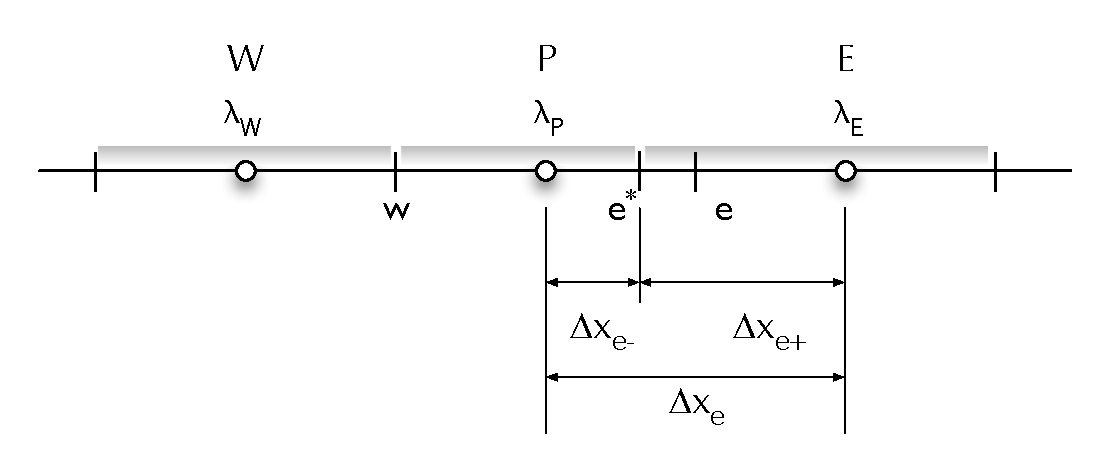
\includegraphics[width=12cm,clip]{face.eps}
\caption{調和平均を用いた拡散項の近似}
\label{fig:diffusive flux}
\end{center}
\end{figure}


これより,熱流束と界面温度は以下のようになる.

\begin{equation}
{{q}'}_{e\mathrm{*}}\,=\,\mathrm{{-}}{\left({\frac{\mathrm{\Delta}{{x}'}_{{e}\mathrm{{+}}}}{{{\mathit{\lambda}}_{E}}}\mathrm{{+}}\frac{\mathrm{\Delta}{{x}'}_{{e}\mathrm{{-}}}}{{{\mathit{\lambda}}_{P}}}}\right)}^{\mathrm{{-}}{1}}\left({{{\mathit{\theta}}'}_{E}\mathrm{{-}}{{\mathit{\theta}}'}_{P}}\right)
\label{eq:difuusive flux at interface:3}
\end{equation}

\begin{equation}
{{\mathit{\theta}}'}_{e\mathrm{*}}\,=\,\frac{{{\mathrm{\varphi}}_{E}}'{{\mathit{\theta}}'}_{E}\mathrm{{+}}{{\mathrm{\varphi}}_{P}}'{{\mathit{\theta}}'}_{P}}{{{\mathrm{\varphi}}_{E}}'\mathrm{{+}}{{\mathrm{\varphi}}_{P}}'}
\label{eq:difuusive flux at interface:4}
\end{equation}

ただし,${\varphi}_{E}^{\prime}\,=\,{\lambda}_{E}/{\Delta x}_{e^{+}}^{\prime},\quad{\varphi}_{P}^{\prime}\,=\,{\lambda}_{P}/{\Delta x}_{e^{-}}^{\prime}$である.

ここで,セル界面が中点$e$の場合を考えてみると,$h^{\prime}$をボクセル幅として,

\begin{equation}
\mathrm{\Delta}{{x}'}_{{e}\mathrm{{+}}}\,=\,\mathrm{\Delta}{{x}'}_{{e}\mathrm{{-}}}\,=\,{h}'/2
\label{eq:difuusive flux at interface:5}
\end{equation}

\begin{equation}
{{q}'}_{e\mathrm{*}}\,=\,\mathrm{{-}}{2}{\left({\frac{1}{{{\mathit{\lambda}}_{E}}}\mathrm{{+}}\frac{1}{{{\mathit{\lambda}}_{P}}}}\right)}^{\mathrm{{-}}{1}}\frac{{{\mathit{\theta}}'}_{E}\mathrm{{-}}{{\mathit{\theta}}'}_{P}}{{h}'}
\label{eq:difuusive flux at interface:6}
\end{equation}

これは,均質媒質のとき拡散流束の標準的な差分近似と同じである.さらに$\lambda_{E}\, \gg \, \lambda_{P}$の場合は$\lambda_{E}$の値が大きいので,\textbf{式(\ref{eq:difuusive flux at interface:6})}は

\begin{equation}
{{q}'}_{e\mathrm{*}}\,=\,\mathrm{{-}}{{\mathit{\lambda}}_{P}}\frac{{{\mathit{\theta}}'}_{E}\mathrm{{-}}{{\mathit{\theta}}'}_{P}}{{{h}'}\slash{2}}
\label{eq:difuusive flux at interface:7}
\end{equation}

となる.\textbf{式(\ref{eq:difuusive flux at interface:7})}は,界面$e^{*}$付近でセル E の温度を$\theta_{E}$と近似した上で片側差分により勾配を近似したことを表している.界面での熱伝導率として調和平均を用いる点に注意する.

\begin{equation}
{{\mathit{\lambda}}_{e\mathrm{*}}} \,=\, {2}\frac{{{\mathit{\lambda}}_{E}}{{\mathit{\lambda}}_{P}}}{{{\mathit{\lambda}}_{E}}\mathrm{{+}}{{\mathit{\lambda}}_{P}}}
\label{eq:difuusive flux at interface:8}
\end{equation}

この方法により,熱拡散係数が異なる媒質間の熱移動を合理的な近似により表現する.

多媒質の場合は,

\begin{equation}
\frac{\theta^{n+1} - \theta^{n}} {\Delta t}
\,=\,
\frac{1}{\rho^{\prime}C} \left[{
\frac{1}{h^{2}} \left\{{
\sum\limits_{j=1}^{\dim\times2} {\left({
\gamma \lambda
}\right)}_{j} \hspace{0.15em}
\theta_{J} \hspace{0.15em}-\hspace{0.15em} \theta_{P} \sum\limits_{j=1}^{\dim\times2}
{\left({
\gamma \lambda
}\right)}_{j}
}\right\}
}\right]
\frac{1}{{u_{\mathit{0}}}^{\prime} L^{\prime}}
\,-\,
\frac{1}{\rho^{\prime}C} \left[{
\frac{1}{h} \sum\limits_{j=1}^{\dim\times2} {
\left({ {-1} }\right)}^{j} \hspace{0.15em}
{\left\{{ 
\left({ {1} - \gamma }\right) q_{BC}^{\prime} 
}\right\}}_{j} 
}\right]
\frac{1}{{u_{\mathit{0}}}^{\prime} \Delta \theta^{\prime}} \,+\, \Theta_{V}
\label{eq:pscalar semi-discrete9}
\end{equation}


%TypeS MM用
ここで$\rho^{\prime}C$は解くべきセルの物性値なので,前処理時に方向インデクスを保存しておく.
境界面を挟む2つのセルのうちどちらが固体要素であるかは,前処理でそのインデクスを特定している.熱伝達境界面をもつインデクスの小さい方のセル(つまり\textbf{図\ref{fig:typeN}}の (a), (b)の両方のパターンともセルj)に熱伝達境界の attribute ID を保持するようにしている.

\textbf{図\ref{fig:typeN}}において,熱境界条件を昇順にサーチし,まずインデクス j を得る.この場合,j+1/2 面が熱伝達形式の境界流束となるので,インデクス j に対して j または j+1 のどちらかが参照側の固体となる.(a) の場合,j 要素が固体なので,j を基準として固体要素の方向を示す値 dir=0 となる.一方 (b) の場合,固体要素は j+1 なので j から見ると,dir=1 である.

多媒質(Multi-Medium, MM)の場合には,セル(i, j)に対する固体要素の参照は (i, j+dir) のように参照できる.一方,流体が単媒質(Single-Medium, SM)の場合には,熱伝達境界条件として与える部分の固体の物性に依存するのみであり,この情報はコンポーネントテーブルから読み取る.
